\chapter{Problemstellung aktiver Fahreingriffe} \label{chap:grundlagen}

%\zitat{But in science the credit goes to the man who convinces the world, \\
%not to the man to whom the idea first occurs.}{Sir Francis Darwin}
\zitat{Es ist nicht genug, zu wissen, man muss auch anwenden; \\
es ist nicht genug zu wollen, man muss auch tun.} {Johann Wolfgang von Goethe}



% Was soll in diesem Kapitel gemacht werden?

In vielen automatisierungstechnischen Anwendungen kommen sog.\ Mehrschicht-\index{Mehrschichtsteuerung} bzw. Mehrebenensteuerungen\index{Mehrebenensteuerung} \cite{lunze2005regelungstechnik} zum Einsatz, die auf dem Prinzip der Dekomposition und Koordination komplexe Aufgabenstellungen\footnote{Als Beispiel sei eine Ablaufsteuerung genannt, die entsprechend einem optimierten Prozess-Grobschema entworfen wird, sodass in Abhängigkeit des aktuellen Prozessschritts eine gezielte Anpassung der nachgeschalteten Steuer- oder Optimierungsalgorithmen erfolgt. Letztere können dann wiederum nach konkretisierten Maßgaben zwischen verschiedenen Sensoren und Aktoren umschalten.%, sodass schließlich, nach dem Durchlauf des Grobschemas, das eigentliche Resultat der Automation erreicht wird.
}  lösen \cite{reinisch1974kybernetische}. Aufgrund hoher Anforderungen an die Funktionsrobustheit und -qualität stellen Fahrerassistenzsysteme hier keine Ausnahme dar. \\
Die Unterteilung moderner Assistenzfunktionen in geeignete Hierarchieebenen ist jedoch keinesfalls trivial, da sie immer von Kompromissen begleitet wird. Infolgedessen wird im vorliegenden Kapitel zunächst das menschliche Verhalten in Form eines etablierten Fahrermodells beschrieben und dazu regelungstechnische Parallelen gezogen. Hierbei stellt sich heraus, dass die Trajektorienoptimierung des Fahrmanövers eine zentrale Rolle einnimmt, da sie nicht nur optimale Fahrzeugbewegungen berechnet, sondern auch durch die Rückführung des Fahrzeug-Istzustands eine qualitativ hochwertige Stabilisierung realisiert. Aufgrund von Einschränkungen bei der praktischen Umsetzung aktorischer Eingriffe ist jedoch in jedem Fall die Trajektorienoptimierung mit einer unterlagerten Regelung zu kombinieren, was später genauer erläutert wird. \\
Der Entwurf und die Umsetzung aktiver Fahreingriffe erfordert generell ein breites Verständnis über die der Fahrerassistenzfunktion zur Verfügung stehenden Schnittstellen zur Aktorik und Sensorik, da erst so das volle Potential bestehender Fahrzeugarchitekturen ausgeschöpft werden kann. Viel wichtiger noch: Sind die grundsätzlichen Zusammenhänge zwischen Eingangs- und Ausgangsdaten verstanden, befähigt das den Entwickler einer Fahrerassistenzfunktion, bei auftauchenden Problemen mit dem jeweiligen Schnittstellenpartner konstruktiv Verbesserungen zu erarbeiten, die das Gesamtsystem auf eine höhere Leistungsebene heben. Aus diesem Grund werden die für die Fahrerassistenzfunktion wichtigsten Aspekte der hinter den etablierten Schnittstellen befindlichen Hardware- und Softwarekomponenten genauer betrachtet. Dabei wird, wann immer möglich, eine zukunftsgerichtete Perspektive eingenommen. \\ %der Schwerpunkt auf zukunftsträchtige Fahrzeugtechnologien gelegt wurde.
%
Ausgangsseitig gehören zu den Schnittstellensystemen die elektromechanische Servolenkung, das elektrohydraulische Bremssystem und der Fahrzeugantrieb. Eingangsseitig handelt es sich um das Sensorcluster (bestehend aus Drehraten- und Beschleunigungssensoren), die Geschwindigkeits- und Schwimmwinkelschätzung, die Module der lokalen und globalen Eigenlokalisierung sowie die Fahrzeugumfeld-Erfassung und -Prädiktion. \\
Abschließend wird im Kapitel die grundsätzliche Herangehensweise bei der Systemaktivierung von Assistenzfunktionen erläutert. Hierzu wird auf das Konzept der sog.\ \emph{Systemzustände einer unvermeidlichen Kollision} und darauf aufbauende subjektive Kritikalitätsmaße zurückgegriffen.
	
	
% Für ein tiefgründiges Verständnis ist es wichtig, auch die unterlagerten Regler zu kennen, die zu einer Beeinflussung des Fahrzeugs führen. Da damit immer eine Dynamik einher geht, die je nach Anwendungsfall vernachlässigt werden kann oder nicht, ist es wichtig auch die physikalischen Zusammenhänge grob zu verstehen.
% -> Übergeordnete Betrachtung, welche sich durch alle anschließenden Kapitel zieht.
%
%Mehrebenen-Optimierung





% Begründung für Schwierigkeit am Beispiel einer Heizung: Hohe Koppelung zwischen Regelung und Führung (nicht so wie Heizungssystem)

\section{Klassifikationsschema der menschlichen Fahraufgabe\index{Fahraufgabe}}

\subsection{Drei-Ebenen-Modell} \label{sec:drei-ebenen-modell}
Entsprechend \cite{handbuchFAS_Donges2012} besteht die übergeordnete Aufgabe des Fahrers darin, das Kraftfahrzeug mit Hilfe von Fahreingriffen unter Berücksichtigung der verfügbaren Information sicher an einen Zielort zu überführen. Eine Unterteilung in hierarchisch verknüpfte Einzelaufgaben kann über das Drei-Ebenen-Modell erfolgen \cite{donges1982aas}, das bereits in der Einleitung in Abb.\,\ref{fig:Navigation_Fuehrung_Stabilisierung} herangezogen wurde und starke Ähnlichkeit mit einem kaskadierten Regelkreis\index{Kaskadenregelung} \cite{graf2003neue} aufweist, s.\ Abb.\,\ref{fig:dreiebenenmodell}. Hierbei umfasst die \textbf{Navigationsaufgabe}\index{Navigationsebene} die Bestimmung einer optimalen Fahrroute in Abhängigkeit des aktuellen Fahrzeugortes und der momentanen Verkehrslage zu diskreten Zeitpunkten, wie zum Fahrtantritt oder Befund einer Straßensperrung. Die Umsetzung der Fahrroute in konkrete Fahrmanöver ist Aufgabe der nachgeschalteten \textbf{Führungsebene}\index{Führungsebene}. Sie wählt unter Berücksichtigung der aktuellen Fahrzeugposition und -bewegung sowie des prädizierten Fahrraums  unter vielerlei Gesichtspunkten, wie Komfort, Verbrauch und Verkehrssicherheit, das zukünftige Fahrmanöver aus. Dessen Realisierung erfolgt mittels motorischer Eingriffe in Lenkrad und Pedalerie und wird aufgrund der hierbei zu unterdrückenden Störungen als \textbf{Stabilisierungsaufgabe}\index{Stabilisierungsebene} bezeichnet. 


%
%
\begin{figure}[h]
	\newcommand{\smallsize}{.85}
	\psfrag{1}[cc][cc][\smallsize]{Navigation}
	\psfrag{2}[cc][cc][\smallsize]{Führung}
	\psfrag{3}[cc][cc][\smallsize]{\parbox[c]{7cm}{\begin{center}Stabilisierung \end{center}}}
	%
	\psfrag{4}[cc][cc][\smallsize]{\parbox[c]{7cm}{\begin{center}Straßennetz \end{center}}}
	\psfrag{5}[cc][cc][\smallsize]{Fahrraum}
	\psfrag{6}[cc][cc][\smallsize]{Fahrzeug}
	%
	\psfrag{7}[cc][cc][\smallsize]{\parbox[c]{7cm}{\begin{center}Lenkung u. \\ Pedalerie \end{center}}}
	%
	\psfrag{m}[cc][cc][1.0]{Planungshorizont}
	\psfrag{n}[cc][cc][1.0]{Reaktionsschnelligkeit}
	%
	\psfrag{a}[cc][cc][1.0]{Fahrer}
	\psfrag{b}[cc][cc][1.0]{Umwelt}
	\psfrag{d}[cc][cc][1.0]{Stellglieder}
	\psfrag{c}[cc][cc][1.0]{Strecke}
	%
	\psfrag{w}[bc][bc][\smallsize]{Fahrzustand 1}
	\psfrag{x}[bc][bc][\smallsize]{Fahrzustand 2}
	\psfrag{y}[bc][bc][\smallsize]{Verkehrsteilnehmer, Hindernisse und relative Fahrspurposition}
	\psfrag{z}[bc][bc][\smallsize]{Aktuelle Fahrspur und Geschwindigkeit}
	\centering
	\includegraphics[width=1.0\textwidth]{2_3-Ebenen-Modell.eps}
	\caption[Modifiziertes Drei-Ebenen-Modell]{Für kritische Fahrsituationen und erfahrene Fahrzeugführer modifiziertes Drei-Ebenen-Modell, vgl.\ \cite{donges1996regelsysteme}}% , vgl.\ \cite{handbuchFAS_Donges2012}}
	\label{fig:dreiebenenmodell}
\end{figure}

Abweichend von der Darstellung des Fahrzeugnormalbetriebs in \cite{handbuchFAS_Donges2012} wird in Abb.\,\ref{fig:dreiebenenmodell} den besonderen Anforderungen bei kritischen Fahrmanövern wie dem Ausweichen Rechnung getragen. Sie verlangen dem Fahrer auf der Führungsebene nicht nur eine genaue Manöverplanung ab, sondern auch eine permanente Berücksichtigung bestimmter Komponenten des aktuellen Fahrzustands (Fahrzustand 2). 
%Letzteres bedarf einer zusätzlichen Erklärung: 
Beim Spurhalten im Normalbetrieb werden nämlich, ungeachtet des Fahrzeugzustands, von der Führungsebene lediglich die Sollspur und die Sollgeschwindigkeit an die Stabilisierungsebene weitergeleitet, die dann Abweichungen von den Sollvorgaben minimiert. Während eines fahrphysikalisch anspruchsvollen Manövers hingegen, muss der Fahrer auf der Führungsebene darauf Rücksicht nehmen, wie sein %durch die Stabilisierungsebene geregeltes 
Fahrzeug tatsächlich reagiert. Das setzt ein gutes Fahrgefühl\footnote{Ein im deutschsprachigen Automobilsport verbreiteter, scherzhafter Ausdruck ist hierfür das sog.\ \emph{Popometer}.} für den Fahrzeugzustand und die Fahrbahnbeschaffenheit voraus. 
Bei rutschigem Untergrund beispielsweise folgt das Fahrzeug häufig nicht so schnell der Lenkbewegung wie erwartet, sodass ein ungeübter Fahrer versucht ist, durch weiteres Einlenken auf der ursprünglichen Ausweichtrajektorie zu bleiben und dadurch eine Verstärkung des sog.\ \emph{Untersteuerns}\index{Untersteuern} riskiert. Der geübte Fahrer hingegen erkennt frühzeitig, dass sein Fahrzeug "`über die Vorderräder schiebt"' und korrigiert das Manöver unter Berücksichtigung des aktuellen Fahrzustands % sowie der geschätzten Fahrbahnbeschaffenheit 
auf der Führungsebene.  Hierdurch entscheidet er sich u.\,U. für ein zum Hindernis hin knapperes, dafür aber fahrphysikalisch realisierbares Ausweichmanöver, mit dem er eine Kollision erfolgreich vermeidet.
Das lässt vermuten, dass der Fahrer mit steigender Erfahrung einen immer größeren Teil des Fahrzustands auf der Führungsebene berücksichtigt.

\subsection{Regelungstechnische Betrachtungsweise}
Aus regelungstechnischer Sicht wird der Fahrer bei seiner Fahraufgabe in jedem Zeitschritt mit einem  Optimalsteuerungsproblem\index{Optimalsteuerung} \cite{foellingeroptimal} konfrontiert, vgl.\ \cite{prokop2001modeling, preusse2001fahrzeugfuhrung}, dessen permanente Lösung bei Berücksichtigung des aktuellen Fahrzustands und der Umgebungsinformation zu einer Stabilisierung des Gesamtsystems führt (s.\ später \abschn{sec:begriffe}).
Das zugrunde gelegte Optimierungskriterium setzt sich i.\,Allg.\ aus Fahrzeit, Verbrauch, Komfort und Sicherheit zusammen. Im Sinne der Optimierungsnebenbedingungen ist zusätzlich zur Fahrphysik auch die jeweils geltende Straßenverkehrsordnung einzuhalten. Die Lösungsfindung einer so abstrakten Aufgabenstellung erfordert jedoch auch vom Menschen die eingangs angesprochene Dekomposition in spezifizierte Teilaufgaben und motiviert das Drei-Ebenen-Modell des vorherigen Abschnitts. Dieses gilt es nun unter dem Aspekt der Optimierung genauer zu beleuchten.

% (unendlichdimensionalen\footnote{Es existieren unendliche viele Möglichkeiten, ein Fahrzeug von A nach B überzuführen.})

In der Mathematik werden bei einem sog.\ Multi-level-Optimierungsansatz große Probleme hierarchisch abstrahiert und in den dabei entstehenden Subproblemen nach teils unterschiedlichen Kriterien optimiert. Auch die Regelungstechnik macht sich die Herangehensweise bei der zuvor erwähnten Mehrebenensteuerung zunutze \cite{lunze2005regelungstechnik}. Sie adressiert damit gleichzeitig drei wichtige und mit den ihr auferlegten Echtzeitanforderungen unmittelbar verknüpfte Aspekte: den Optimierungshorizont\index{Optimierungshorizont}\footnote{Zeitintervall in die Zukunft, auf dem das Streckenverhalten betrachtet wird.}, die Zykluszeit\index{Zykluszeit}\footnote{Verstreichende Zeitspanne bis in der Optimierung die neue Messinformation Berücksichtigung findet.} und die Systemzustandsdimension\index{Systemzustand}\footnote{Anzahl der dem Optimierungsproblem zugrunde gelegten Modell-Systemzustände}. Ein weitreichender Optimierungshorizont ist für das Auffinden einer langfristig guten Strategie erforderlich und sollte sich an den langsamsten Dynamiken der Strecke orientieren. Die Systemstabilität des durch die Zustandsrückführung in der permanenten Optimierung geschlossenen Regelkreises hingegen verlangt eine so kurze Zykluszeit, dass auch die schnellsten Streckendynamiken berücksichtigt und damit robust stabilisiert werden können. Aufgrund der beschränkten Rechenleistung eines jeden Computers steht aber ein langer Optimierungshorizont mit einer kurzen Zykluszeit im Widerspruch. %\footnote{Eine Ausnahme stellen sog.\ Linear-quadratische-Probleme dar, s.\ Abschn.\,\ref{sec:lqr}, deren Lösung trotz eines unendlichen Optimierungshorizonts eine kontinuierliche Rückführung ermöglichen.}, 
Er kann durch eine hierarchische bzw.\ kaskadische Problemaufteilung, wenn auch kompromissbehaftet, aufgelöst werden, indem in der Signalkette sukzessive immer mehr Zustände des Fahrzeugs berücksichtigt werden. \\
Konkret spiegelt sich das im Drei-Ebenen-Modell darin wider, dass auf \textbf{Navigationsebene}\index{Navigationsebene}
\begin{itemize}
\item die Fahrzeit und der Verbrauch optimiert werden, 
\item die Fahrphysik zu vernachlässigen ist (Abstraktion auf Punktbewegung), 
\item sich die Zykluszeit auf wenige Optimierungen pro Minute beschränkt und 
\item sich der Optimierungshorizont über mehrere Stunden erstrecken kann. 
\end{itemize}
Das Ergebnis ist eine Fahrroute, welche der Optimierung auf Fahrzeugführungsebene als Referenz dient und weiter verfeinert werden muss. \\
Die \textbf{Fahrzeugführungsebene}\index{Fahrzeugführungsebene} wiederum setzt sie nach Möglichkeiten um und optimiert dabei die zukünftige Fahrzeugbewegung
\begin{itemize}
\item unter Sicherheits- und Komfortaspekten (primär),
\item unter Berücksichtigung der Fahrphysik,
\item auf einem Optimierungshorizont von wenigen Sekunden, 
\item dafür aber so häufig wie möglich, um schnell auf den veränderlichen Verkehr und den Fahrzeugzustand reagieren zu können.
\end{itemize}
%um der schnell wechselnden Fahrsituation Rechnung zu tragen. 
Das Resultat stellt ein optimiertes Fahrmanöver dar, das von der \textbf{Stabilisierungsebene}\index{Fahrzeugführungsebene} trotz Modellunsicherheiten hinreichend genau mittels Eingriffen in die Fahrzeugquer- und -längsdynamik auszuführen ist.

Da sowohl auf der Stabilisierungsebene als auch auf der darüber liegenden Führungsebene der Fahrzeugzustand rückgeführt wird, übernimmt auch die Führungsebene einen Teil der Stabilisierungsaufgabe. 
Um etwaige Wechselwirkungen innerhalb der Module eines Fahrerassistenzsystems erkennen und beurteilen zu können, wird die Thematik noch genauer in Kapitel~\ref{chap:stabilisierung} beleuchtet. %mit einem allgemeinen regelungstechnischen Fokus 
%Die mathematische Behandlung der Stabilität modellprädiktiver Regelkreise erfolgt dann in 

\section{Begriffserläuterungen der Regelungstechnik und Robotik} \label{sec:begriffe}
Im Kontext moderner Fahrerassistenzsysteme häufig anzutreffende Termini sind \emph{Trajektorien-}\index{Trajektorienplanung} und \emph{Pfadplanung}\index{Pfadplanung},  welche der Regelungstechnik und Robotik entstammen. Da die vorliegende Arbeit ihren Fokus auf die Optimierung auf Fahrzeugführungsebene legt, soll an der Stelle dem Leser deren Ursprungsgedanke vermittelt und ein Überblick über eng damit verbundene Begrifflichkeiten verschafft werden. Es sei jetzt schon angemerkt, dass in der Fachliteratur aufgrund unterschiedlicher Forschungsschwerpunkte die Verwendung der Begriffe nicht einheitlich erfolgt.
%Darauf aufbauend wird anschließend das für die Praxisanwendung wichtige Zusammenspiel von Optimierung und Regelung genauer beleuchtet.
\subsection{Trajektorien- und Pfadplanung} \label{sec:begriff_tp}
% Oft nicht optimal, einmalig und impliziert damit nachgelagerte Reglung
Die industrielle Praxis der Regelungstechnik ist geprägt von sog.\ Arbeitspunkten und deren Wechsel \cite{lunze2005regelungstechnik, hagenmeyer2004flachheitsbasierter}. Hierbei wird über eine lange Zeit hinweg eine konstante Referenz vorgegeben, deren Stabilisierung Aufgabe der Regelung ist (\emph{Festwertregelung}). Wird nun zwischen weit auseinander liegenden Arbeitspunkten abrupt umgeschaltet, so läuft der Regler Gefahr, in die (im Reglerentwurf oftmals unmodellierten) Stellgrößenbeschränkungen zu laufen, sodass sich die Strecke destabilisiert (\emph{Regler-} bzw.\ \emph{Strecken-Windup} \cite{hippe2004neue}). Zur Vermeidung solcher Effekte %der mit solchen Arbeitspunktwechseln verbundenen Stöße auf die Strecke und möglicherweise gar auftretenden Destabilisierung des Regelkreises , 
wird der zeitliche Sollverlauf der Führungsgröße zwischen den Arbeitspunkten entsprechend der verfügbaren Stellgröße gewählt \cite{hagenmeyer2004flachheitsbasierter} und die Festwertregelung\index{Festwertregelung} durch eine (asymptotische) \emph{Folgeregelung}\index{Folgeregelung} ersetzt, s.\ \abb{fig:arbeitspunktwechsel_tp_prinzip}. Zur Beschreibung des Sollverlaufs $\bs x_r(t)$ (hier für den Systemzustand) reicht häufig ein Referenzpolynom entsprechender Ordnung, bei dem die Transitionszeit $T_\text{trans}$ so minimiert wird, dass die Beschränkungen für die Stellgröße $\bs u$ (in Abb.\,\ref{fig:arbeitspunktwechsel_tp} auf $\bs u_{\min}$) nicht aktiv werden, s.\ \zB \cite{zeitz2010differenzielle}. %Im Allgemeinen kommen dabei Methoden der Parameteroptimierung zum Einsatz, was auch als Statische Optimierung \cite{foellingeroptimal} bezeichnet wird. %, s.\ Kap.\,\ref{chap:statische_Optimierung}.
%Die Stabilisierung der sich zeitlich verändernden Referenztrajektorie $x_r(t)$ wird über eine nachgelagerte Folgeregelung \cite{hagenmeyer2004flachheitsbasierter} realisiert, s.\ hierzu später Abschn.\ref{todo}. 
Bemerkenswert ist an der Stelle, dass keine Rückkopplung des Systemzustands~$\bs x$ auf der Planungsebene stattfindet, mit Ausnahme der Systeminitialisierung (s.\ $\bs x_0$ in \abb{fig:arbeitspunktwechsel_tp_prinzip}), etwa beim Anfahren. Mit anderen Worten: Die Trajektorienplanung verlässt sich darauf, dass die unterlagerte Regelung korrekt arbeitet.\\
Der Begriff "`Planung"' impliziert jedoch keinesfalls, dass immer eine Optimierung stattfindet. Für einfache Problemstellungen reicht es nämlich aus, die funktionale Darstellung des Übergangs $\bs x_r(t)$ so zu wählen, dass nach Festlegung der Stetigkeitsanforderung und Transitionszeit kein Freiheitsgrad für eine Optimierung verbleibt. Erfordert die regelungstechnische Aufgabenstellung jedoch eine (möglicherweise zyklische) Optimierung, impliziert die Verwendung des Begriffs "`Trajektorienplanung"' dann \iA den Einsatz einer \emph{nachgelagerten} Folgeregelung, s.\ Absch.\,\ref{sec:asymptotische_folgeregelung}.\\

\begin{figure}[h]
\newcommand{\smallsize}{.85}
	\psfrag{1}[cr][cr][1.0]{$\bs x(t)$}
	\psfrag{2}[tc][tc][1.0]{$t$}
	\psfrag{u}[cr][cr][1.0]{$\bs u(t)$}
	\psfrag{m}[cr][cr][1.0]{$\bs u_{\min}$}
	\psfrag{a}[cc][cc][\smallsize]{\parbox[c]{7cm}{\begin{center}Trajektorien-\\ planung \end{center}}}
	\psfrag{b}[cc][cc][\smallsize]{\parbox[c]{7cm}{\begin{center}Folge-\\ regelung \end{center}}}
	\psfrag{c}[cc][cc][\smallsize]{\parbox[c]{7cm}{\begin{center}Strecke \end{center}}}
	\psfrag{x}[bc][bc][1.0]{$\bs x_r$}
	\psfrag{r}[bc][bc][1.0]{$\bs u$}
	\psfrag{z}[bc][bc][1.0]{$\bs x$}
	\psfrag{y}[cl][cl][1.0]{$\bs x_0$}
	\centering
	\includegraphics[width=.8\textwidth,clip, trim = 0cm 0cm 0cm 0cm]{2_Prinzip_Trajektorienplanung.eps} \\
	  	\caption{Arbeitsweise einer Trajektorienplanung mit Folgeregelung}
    \label{fig:arbeitspunktwechsel_tp_prinzip}
\end{figure} 
%
\begin{figure}[h]
\newcommand{\smallsize}{.85}
	\psfrag{1}[cr][cr][1.0]{$\bs x(t)$}
	\psfrag{2}[tc][tc][1.0]{$t$}
	\psfrag{u}[cr][cr][1.0]{$\bs u(t)$}
	\psfrag{m}[cr][cr][1.0]{$\bs u_{\min}$}
	\psfrag{T}[bc][bc][1.0]{$T_\text{trans}$}
	\psfrag{a}[cc][cc][\smallsize]{\parbox[c]{7cm}{\begin{center}Trajektorien-\\ planung \end{center}}}
	\psfrag{b}[cc][cc][\smallsize]{\parbox[c]{7cm}{\begin{center}Folge-\\ regelung \end{center}}}
	\psfrag{c}[cc][cc][\smallsize]{\parbox[c]{7cm}{\begin{center}Strecke \end{center}}}
	\psfrag{x}[bc][bc][1.0]{$\bs x_r$}
	\psfrag{r}[bc][bc][1.0]{$\bs u$}
	\psfrag{z}[bc][bc][1.0]{$\bs x$}
	\psfrag{y}[cl][cl][1.0]{$\bs x_0$}
	\centering
  	\includegraphics[width=.47\textwidth,clip, trim = 0cm 0cm 0cm 0cm]{2_arbeitspunktwechsel_tp.eps} 
	\hspace{.5cm}
		 \includegraphics[width=.47\textwidth,clip, trim = 0cm 0cm 0cm 0cm]{2_arbeitspunktwechsel_tp_u.eps}
  	\caption[Signalverläufe bei der Trajektorienplanung]{Signalverläufe eines Arbeitspunktwechsels bei der Trajektorienplanung mit Folgeregelung: Geplante Referenzverläufe des Zustands und der Stellgröße in Weiß, tatsächliche Verläufe in Schwarz; $T_\text{trans}$ bezeichnet die Transitionszeit zwischen den Arbeitspunkten und $\bs u_{\min}$ die (untere) Stellgrößensättigung}
    \label{fig:arbeitspunktwechsel_tp}
\end{figure}
Die Robotik verwendet den Begriff "`Trajektorienplanung"' jedoch in einem etwas anderen Kontext. Häufig kann die Roboterumgebung als statisch angesehen werden, sodass die Zeit $t$ eine untergeordnete Rolle spielt. Wenn nämlich die Roboterdynamik weitgehend geschwindigkeitsunabhängig ist, dann kommt es vielmehr auf die richtige Abfolge der Stelleingriffe an (häufig in Abhängigkeit der zurückgelegten Wegstrecke $s$, welche dann die unabhängige Variable darstellt), und es wird von \emph{Pfad-}\index{Pfadplanung} oder \emph{Bahnplanung}\index{Bahnplanung} gesprochen \cite{latombe1990robot, lavalle2006pa}. Der Begriff "`Trajektorienplanung"' wird nur dann herangezogen, wenn das Planungsergebnis in Abhängigkeit von der Zeit vorliegt. Im einfachsten Fall reicht es hierfür aus, den Pfad mit einem Geschwindigkeitsprofil zu überlagern \cite{lavalle2006pa}.

%Auch wenn hierbei häufig von $t$ zu einer anderen unabhängigen Variablen wie der auf dem berechneten Pfad zurückgelegten Wegstrecke $s$ übergegangen wird, ändert sich grundsätzlich nichts an den zuvor beschriebenen Problemstellungen und Herangehensweisen. Lediglich die Stabilisierung des Manövers erfordert in bestimmten Situationen zusätzlich die Bestimmung des aktuellen $s$ durch Projektion (s.\ hierzu später Abschn.\ref{sec:projektion}).




\subsection{Optimalsteuerung} \label{sec:def_optimalsteuerung}
Treten beim Arbeitspunktwechsel zu den Stellgrößenbeschränkungen\index{Stellgrößenbeschränkung} zusätzlich Gütekriterien wie die Minimierung der Stellenergie hinzu, oder soll die verfügbare Stellgröße besser ausgenutzt werden, um die Transitionszeit weiter zu verkürzen, so wird in der Regelungstechnik die Methode der \emph{Optimalsteuerung}\index{Optimalsteuerung} \cite{foellingeroptimal} angewandt\. %, s.\ Kap.\,\ref{chap:dynamische_Optimierung_direkt}, \ref{chap:dynamische_Optimierung_indirekt} und \ref{chap:dynamische_Optimierung_dynamisch}.  %\footnote{Viele numerischen Methoden der dynamischen Optimierung approximieren allerdings das Problem durch ein Optimierung eingesetzt}.
Im Mittelpunkt steht hierbei die Optimierung des Modellverhaltens als Reaktion auf das Systemeingangssignal $\bs u$. Genauer gesagt wird nicht nur über eine endliche Anzahl von Parametern optimiert, etwa über Polynomkoeffizienten, sondern die optimale Steuertrajektorie $\bs u^\ast(t)$ als solche gesucht. Dies stellt ein unendlichdimensionales Problem dar, sodass auch die Begriffe \emph{Strukturoptimierung}, \emph{Dynamische Optimierung} oder \emph{Unendlich-dimensionale Optimierung} verwendet werden \cite{foellingeroptimal}. \\
Wie die Methodenbezeichnung vermuten lässt, handelt es sich bei $\bs u^\ast$ zunächst um eine reine Steuerung, die entsprechend Abb.\,\ref{fig:arbeitspunktwechsel_optimalsteuerung_prinzip} als $\bs u(t) = \bs u^\ast(t)$ direkt auf die Strecke gegeben werden kann. Das optimale Ergebnis wird aber nur in Abwesenheit von Störungen und Modellfehlern erreicht (s.\ \abb{fig:arbeitspunktwechsel_optimalsteuerung}). Da bei der Berechnung jedoch die optimale Modelltrajektorie $\bs x^\ast(t)$ abfällt, kann sie im Sinne der Trajektorienplanung (s.\ Abschn.\,\ref{sec:begriff_tp}) als Referenz $\bs  x_r(t) = \bs x^\ast(t)$ herangezogen und mit einer nachgeschalteten Folgeregelung entsprechend Abb.\,\ref{fig:arbeitspunktwechsel_tp} stabilisiert werden. \\
Auch zur Erfüllung der Fahraufgabe muss, wie eingangs erwähnt, in jedem Zeitschritt ein Optimalsteuerungsproblem gelöst werden, was im Assistenzsystem über die in den Kap.\,\ref{chap:dynamische_Optimierung_dynamisch}, \ref{chap:dynamische_Optimierung_direkt} und \ref{chap:dynamische_Optimierung_indirekt} etablierten Methoden erfolgt.
\begin{figure}[h]
\newcommand{\smallsize}{.85}
	\psfrag{1}[cr][cr][1.0]{$\bs x(t)$}
	\psfrag{2}[tc][tc][1.0]{$t$}
	\psfrag{u}[cr][cr][1.0]{$\bs u(t)$}
	\psfrag{r}[bc][bc][1.0]{$\bs u^\ast$}
	\psfrag{m}[cr][cr][1.0]{$\bs u_{\min}$}
	\psfrag{z}[bc][bc][1.0]{$\bs x$}
	\psfrag{y}[cl][cl][1.0]{$\bs x_0$}
	\psfrag{b}[cc][cc][\smallsize]{\parbox[c]{7cm}{\begin{center}Optimal-\\ steuerung \end{center}}}
	\psfrag{c}[cc][cc][\smallsize]{\parbox[c]{7cm}{\begin{center}Strecke \end{center}}}
	\centering
		\includegraphics[width=.6\textwidth,clip, trim = 0cm 0cm 0cm 0cm]{2_Prinzip_Optimalsteuerung.eps} \\
  	\caption[Arbeitsweise der Optimalsteuerung]{Arbeitsweise der Optimalsteuerung \cite{foellingeroptimal}}
    \label{fig:arbeitspunktwechsel_optimalsteuerung_prinzip}
\end{figure} 
%
\begin{figure}[h]
\newcommand{\smallsize}{.85}
	\psfrag{1}[cr][cr][1.0]{$\bs x(t)$}
	\psfrag{2}[tc][tc][1.0]{$t$}
	\psfrag{u}[cr][cr][1.0]{$\bs u(t)$}
	\psfrag{m}[cr][cr][1.0]{$\bs u_{\min}$}
	\psfrag{z}[bc][bc][1.0]{$\bs x$}
	\psfrag{y}[cl][cl][1.0]{$\bs x_0$}
	\psfrag{b}[cc][cc][\smallsize]{\parbox[c]{7cm}{\begin{center}Optimal-\\ steuerung \end{center}}}
	\psfrag{c}[cc][cc][\smallsize]{\parbox[c]{7cm}{\begin{center}Strecke \end{center}}}
	\centering
  	\includegraphics[width=.47\textwidth,clip, trim = 0cm 0cm 0cm 0cm]{2_arbeitspunktwechsel_optimalsteuerung.eps}
	\hspace{.5cm}
		\includegraphics[width=.47\textwidth,clip, trim = 0cm 0cm 0cm 0cm]{2_arbeitspunktwechsel_optimalsteuerung_u.eps}
  	\caption[Signalverläufe der Optimalsteuerung]{Signalverläufe der Optimalsteuerung: Geplante Referenzverläufe des Zustands und der Stellgröße in Weiß, tatsächliche Verläufe in Schwarz; $\bs u_{\min}$ bezeichnet die (untere) Stellgrößensättigung; Aufgrund von Störungen kommt es zu einer merklichen Endabweichung zwischen geplanter und tatsächlicher Trajektorie.}
    \label{fig:arbeitspunktwechsel_optimalsteuerung}
\end{figure} 

\subsection{Optimale und Modellprädiktive Regelung} \label{sec:def_modellpraediktive_Regelung}
Das Fahrzeugumfeld ist stetig von nur schwer vorhersehbarem Wechsel geprägt, und damit ändert sich auch ständig das Optimierungsproblem. Ausgedehnte Fahreingriffe erfordern deshalb eine permanente Optimierung, die der neuen Umfeldinformation Rechnung trägt. 
Wird in der Regelungstechnik ein Optimalsteuerungsproblem ausgehend vom aktuellen Systemzustand $\bs x$ permanent gelöst  
%hierbei ausgehend vom aktuellen Systemzustand $x$ optimiert 
und das Ergebnis auf die Regelstrecke gegeben, so ergibt sich aufgrund der Rückführung ein geschlossener Regelkreis, s.\ Abb.\,\ref{fig:arbeitspunktwechsel_optimaleregelung_prinzip} und \ref{fig:arbeitspunktwechsel_optimaleregelung}. Anschaulich erfolgt die Stabilisierung des Systems über die Rückführung dadurch, dass der Systemzustand $\bs x$ die Wirkung der vorangegangen Störungen widerspiegelt \cite{foellingeroptimal}. Hierbei sind sich zufällige, impulsförmige Störungen vorzustellen, die das prädizierte Streckenverhalten nicht in Frage stellen. Im Unterschied zur Stabilisierung einer Trajektorie mittels nachgeschalteter Folgeregelung, die das System bei Impulsstörungen lediglich (mit hohen Stellgrößen!) auf die alte Referenz $\bs x_r(t)$ zurückführt, wird hier der aktuell gemessene Systemzustand optimal berücksichtigt. \\
Kann eine sehr schlanke, ggf. sogar analytische Lösung für das der Regelung zugrundeliegende Optimalsteuerungsproblem gefunden werden, so wird (tendenziell) von \emph{Optimaler Regelung}\index{Optimalregelung}  \cite{foellingeroptimal} gesprochen. Die Verwendung des Begriffs \emph{Modellprädiktive Regelung}\index{Modellprädiktiver Regelkreis} (\emph{model predictive control}, MPC) \cite{Findeisen2003} hingegen deutet auf ein für analytische Methoden zu schwieriges Optimalsteuerungsproblem hin, das in jedem Schritt numerisch auf einem verkürzten und sich zeitlich mitbewegenden\footnote{Es ist daher auch die Rede von \emph{receding horizon control}.} Optimierungshorizont\index{Optimierungshorizont} gelöst werden muss. 
Das trifft im Übrigen auch auf die Optimierung von Fahrmanövern zu, s.\ Abschn.\,\ref{sec:unendlichdim_opt}. Anhaltende, nicht vernachlässigbare Störungen und Modellfehler erfordern jedoch zusätzliche Maßnahmen, die genauer in Abschn.\,\ref{sec:unterlagerteRegelung} 
diskutiert werden.




\begin{figure}[h]
\newcommand{\smallsize}{.85}
	\psfrag{1}[cr][cr][1.0]{$\bs x(t)$}
	\psfrag{2}[tc][tc][1.0]{$t$}
	\psfrag{3}[cc][cc][.8]{$(\ldots)$}
	\psfrag{u}[cr][cr][1.0]{$\bs u(t)$}
	\psfrag{r}[bc][bc][1.0]{$\bs u^\ast$}
  \psfrag{m}[cr][cr][1.0]{$\bs u_{\min}$}
	\psfrag{z}[bc][bc][1.0]{$\bs x$}
	\psfrag{b}[cc][cc][\smallsize]{\parbox[c]{7cm}{\begin{center}Modellprädiktive\\ Regelung \end{center}}}
	\psfrag{c}[cc][cc][\smallsize]{\parbox[c]{7cm}{\begin{center}Strecke \end{center}}}
	\centering
			\includegraphics[width=.6\textwidth,clip, trim = 0cm 0cm 0cm 0cm]{2_Prinzip_Optimale_Regelung.eps}
  	\caption[Arbeitsweise der modellprädiktiven Regelung]{Arbeitsweise der modellprädiktiven Regelung, vgl.\ \cite{foellingeroptimal}}
    \label{fig:arbeitspunktwechsel_optimaleregelung_prinzip}
\end{figure}

\begin{figure}[h]
\newcommand{\smallsize}{.85}
	\psfrag{1}[cr][cr][1.0]{$\bs x(t)$}
	\psfrag{2}[tc][tc][1.0]{$t$}
	\psfrag{3}[cc][cc][.8]{$(\ldots)$}
	\psfrag{u}[cr][cr][1.0]{$\bs u(t)$}
	\psfrag{r}[bc][bc][1.0]{$\bs u$}
  \psfrag{m}[cr][cr][1.0]{$\bs u_{\min}$}
	\psfrag{z}[bc][bc][1.0]{$\bs x$}
	\psfrag{b}[cc][cc][\smallsize]{\parbox[c]{7cm}{\begin{center}Modellprädiktive\\ Regelung \end{center}}}
	\psfrag{c}[cc][cc][\smallsize]{\parbox[c]{7cm}{\begin{center}Strecke \end{center}}}
	\centering
  	\includegraphics[width=.47\textwidth,clip, trim = 0cm 0cm 0cm 0cm]{2_arbeitspunktwechsel_optimaleregelung.eps}
	\hspace{.5cm}
		\includegraphics[width=.47\textwidth,clip, trim = 0cm 0cm 0cm 0cm]{2_arbeitspunktwechsel_optimaleregelung_u.eps}
  	\caption[Signalverläufe der modellprädiktiven Regelung]{Signalverläufe der modellprädiktiven Regelung, vgl.\ \cite{graichen2014SkriptOpt}: Auf einem sich zeitlich verschiebenden Horizont zyklisch geplante Referenzverläufe des Zustands und der Stellgröße in Weiß, tatsächliche Verläufe in Schwarz; $\bs u_{\min}$ bezeichnet die (untere) Stellgrößensättigung}
    \label{fig:arbeitspunktwechsel_optimaleregelung}
\end{figure}



\section{Aktorik\index{Aktorik} und Stellgrößen\index{Stellgröße}} \label{sec:aktuatorik}
Bei dem Entwurf und der Implementierung fahraktiver Sicherheits- und Komfortfunktionen ist ein tiefergehendes Verständnis über die technische Realisierung der Aktorikeingriffe von Lenkung, Bremse und Gas unverzichtbar. Insbesondere die mit der eingesetzten Hardware eng verkoppelten Möglichkeiten und Einschränkungen der Stellgrößenüberlagerung mit dem Fahrer sind von substantieller Bedeutung, da das Fahrerassistenzsystem, zumindest für kurze Zeit, mit dem Fahrer kooperiert. Darüber hinaus haben sich bestimmte Regelgrößen in den jeweiligen Aktoriksteuergeräten etabliert, die als vereinheitlichte Schnittstellen der Fahrerassistenz zur Verfügung stehen und somit die Stellgröße des überlagerten Regelkreises repräsentieren. Die Kenntnis über diese abstrahierten Schnittstellen und die mit ihren unterlagerten Reglern verbundenen Dynamiken erleichtern den Funktionsentwurf enorm, da sie "`böse Überraschungen"' verhindern. Darum wird im Folgenden der Aufbau und die Funktionsweise moderner Lenk-, Brems- und Antriebssysteme aus Fahrerassistenzsicht genauer beleuchtet.

\subsection{Lenkaktorik}
Im Pkw-Bereich kann in den letzten Jahren ein stetiger Übergang von hydraulischen  hin zu elektrischen Lenksystemen\index{elektrisches Lenksystem} (\emph{Electric Power Steering}, EPS) verzeichnet werden \cite{karch2007mechatronische}. Hierbei wird die herkömmliche Lenkunterstützung des druckbeaufschlagten Servoöls durch die Magnetfeldkraft des Elektromotors ersetzt. % (s.\ Abschn.\,\ref{sec:eps_Aufbau}). 
Das bringt den Vorteil mit sich, dass nur dann Energie benötigt wird, wenn der Fahrer auch lenkt und der Verbrauch erheblich gesenkt\footnote{Bei einem Mittelklassefahrzeug mit einem \unit[2,0]{l} Benzinmotor können Verbrauchseinsparungen von bis zu \unit[0,5]{l}\,/\unit[100]{km} erreicht werden \cite{pfeffer2013lenkungshandbuch}.} werden kann. \\ 
Gleichzeitig eröffnet die Ansteuerung des Elektromotors die Möglichkeit, dem Fahrer ein haptisches Feedback über das Lenkrad zu geben oder gar direkt die Lenkbewegung vorzugeben\footnote{Bei hydraulischen Lenksystemen erfordert das zusätzlich einen sog.\, Handmomentensteller, der auf hydraulische oder elektrische Weise das Fahrerhandmoment am Lenkrad nachahmt.}. Damit ist die EPS das wichtigste Stellglied der Fahrerassistenz zur Beeinflussung der Fahrzeugquerdynamik. % und wird im Folgenden genauer beleuchtet. 
\subsubsection{Systemkomponenten und -aufbau} \label{sec:eps_Aufbau}
Wie in Abb.\,\ref{fig:eps_funktionsweise} dargestellt, kann die Lenkunterstützung\index{Lenkunterstützung} des Elektromotors (M) je nach Gewichtung der Einflussfaktoren Kosten, Energieverbrauch, Akustik und Bauraum an der Lenksäule oder Zahnstange über ein Servogetriebe (G$_\text{M}$) eingeleitet werden. Über eine Drehmomentsensorik (S) wird das Fahrerhandmoment ($M_\text{Hand}$) gemessen und mittels der im Steuergerät befindlichen Software in das Motormoment ($M_\text{Motor}$) umgerechnet. Über die meist ebenfalls im Steuergerät integrierte Leistungselektronik erfolgt die entsprechende Ansteuerung des Motors \cite{pfeffer2013lenkungshandbuch}. Die hohe Flexibilität einer Steuergerätesoftware ermöglicht hierbei, den Unterstützungsgrad in Abhängigkeit des Fahrzustands nahezu beliebig zu variieren. \\
Beim Einsatz von variablen Übersetzungen im Zahnstangenlenkgetriebe (G$_\text{H}$) kann (abhängig vom Lenkwinkel) dem gesteigerten Lenkwinkelbedarf beim Parkieren und Rangieren Rechnung getragen werden. %Zur deutlichen Verbesserung des Gierverhaltens (Drehbewegung um die Hochachse, s.\ später Abschnitt \ref{sec:fahrzeugmodellierung}) auch bei mittleren Geschwindigkeiten kann, wenn auch mit hohen Kosten verbunden, ein Lenkwinkelüberlagerungssystem eingesetzt werden.
Eine noch höhere Flexibilität wird durch ein, wenn auch mit hohen Kosten verbundenes, Lenkwinkelüberlagerungssystem realisiert. Es sorgt durch einen weiteren Elektromotor in Kombination mit einem entweder vor %Audi
 oder unmittelbar nach dem Lenkmomentsensor installierten Winkelüberlagerungsgetriebe %BMW
für eine zusätzliche Verdrehung in der Lenksäule, sodass nahezu beliebige Übersetzungen realisiert werden können. \\
Die beschriebenen und weitgehend entkoppelten Einflussmöglichkeiten auf Lenkmoment und Lenkwinkel bzw.\ Spurstange und Radwinkel der Räder führen dazu, dass bereits heute Lenkfreiheitsgrade geschaffen werden, die einem Steer-by-Wire-System\index{steer-by-wire} \cite{odenthal2003ubertragung} sehr nahe kommen \cite{karch2007mechatronische}. 

\begin{figure}[ht]
	\psfrag{M}[cc][cc][1.0]{M}
	\psfrag{G}[cc][cc][1.0]{G$_\text{M}$}
	\psfrag{I}[cc][cc][1.0]{G$_\text{H}$}
	\psfrag{S}[cc][cc][1.0]{S}
	\psfrag{3}[tl][tl]{$M_\text{Motor}$}
	\psfrag{4}[cl][cl]{$M_\text{Hand}$}
	\psfrag{5}[cb][cb]{$F_z$}
	\psfrag{6}[tl][tl]{$M_\text{Motor}$}
\centering
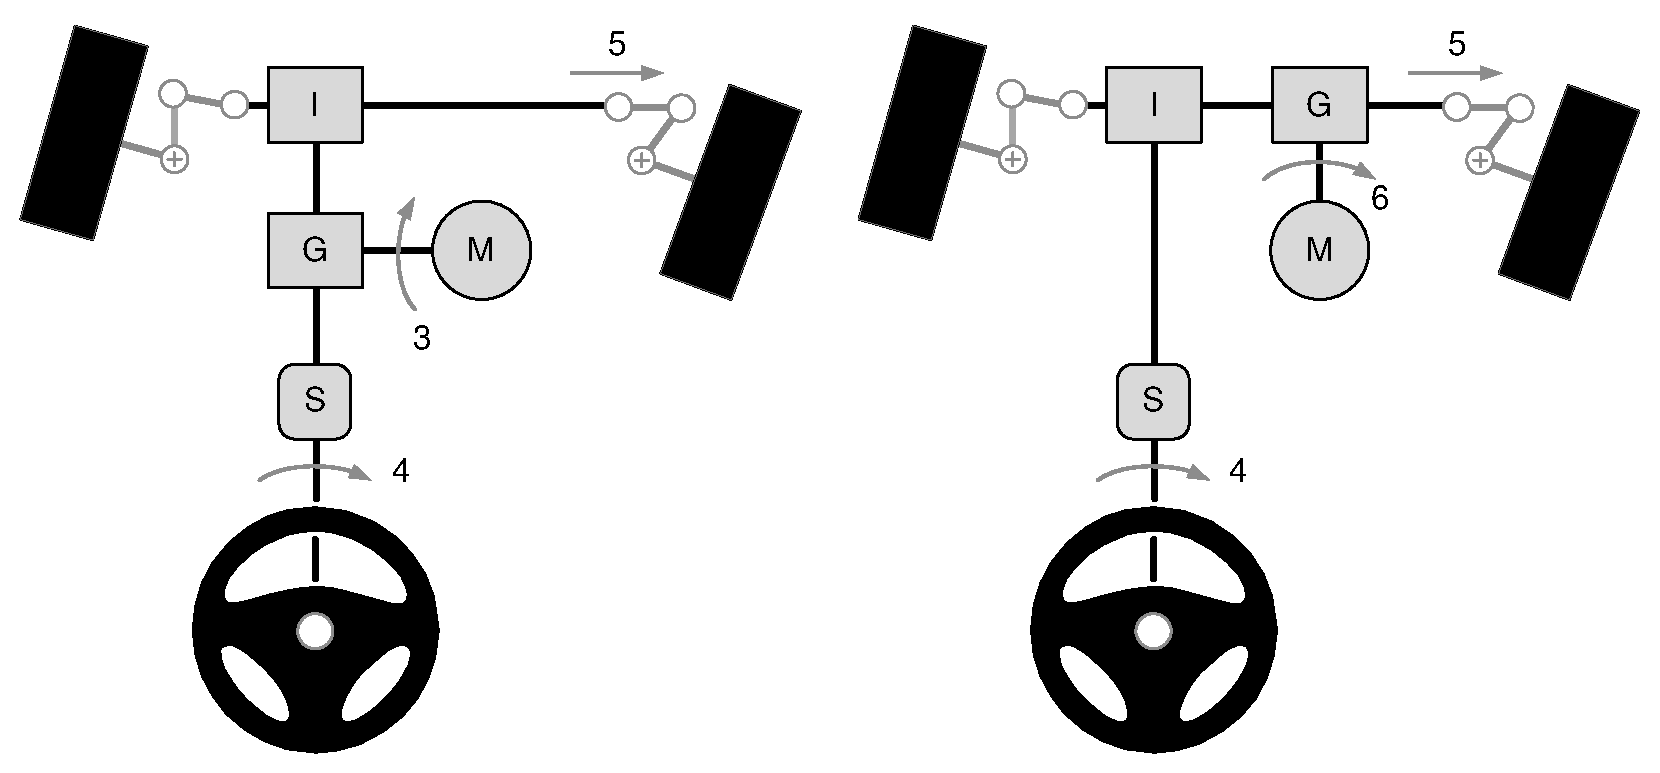
\includegraphics[width=1.0\textwidth,clip, trim = 0cm 0cm 0cm 0cm]{2_EPS_Komponenten.eps}
 \caption[Lenksäulen-basiertes und Zahnstangen-basiertes EPS-System]{Lenksäulen-basiertes (links) und Zahnstangen-basiertes EPS-System (rechts) mit Motor (M), Handmomentsensor (S), Servogetriebe (G$_\text{M}$) und Zahnstangenlenkgetriebe (G$_\text{H}$), vgl.\ \cite{pfeffer2013lenkungshandbuch}}
 \label{fig:eps_funktionsweise}
\end{figure} 

\subsubsection{Funktionsweise} \label{sec:eps_funktionsweise}
%\textbf{Klassisches Regelungskonzept} \\
Das dem herkömmlichen Hydrauliklenksystem nachempfundene Regelungsprinzip zur Bestimmung des elektrischen Servomoments beruht auf der progressiven Verstärkung des Handmoments. Wie in Abb.\,\ref{fig:eps_grundfunktion} dargestellt, wird das gemessene Handmoment entsprechend einem geschwindigkeitsabhängigen Kennfeld $K(v)$ überproportional verstärkt und damit über das Servogetriebe das Lenksystem beaufschlagt. Hierdurch wird erreicht, dass sich (unter Vernachlässigung von Reibungseffekten) die stationäre Zahnstangenkraft $F_z$, Abb.\,\ref{fig:eps_funktionsweise}, zu
\begin{align}
\label{equ:eps_f_z_0}
	F_z &= i_\text{Hand} M_\text{Hand} + i_\text{Motor} M_\text{Motor} \\
	\label{equ:eps_f_z}
	&= i_\text{Hand} M_\text{Hand} + i_\text{Motor} K(v;M_\text{Hand}) 
\end{align}
ergibt, wobei $i_\text{Hand}$ und $i_\text{Motor}$ die jeweiligen Gesamtübersetzungen der Momente auf die Zahnstangenkraft darstellen. \\
Die Höhe des Unterstützungsgrads aus dem Kennfeld hat einen entscheidenden Einfluss auf das Lenkgefühl. So wird durch dessen Geschwindigkeitsadaption hin zu einer reduzierten Servounterstützung bei höheren Geschwindigkeiten erreicht, dass der Fahrer vermehrt die Zahnstangenkraft an der Lenkung verspürt und damit eine differenzierte Rückmeldung von der Fahrbahn erhält. Beim Parkieren und Rangieren hingegen, wo die Zahnstangenkräfte am höchsten ausfallen, kann auf diese Informationsquelle verzichtet werden, sodass zugunsten des Komforts der Unterstützungsgrad deutlich erhöht wird \cite{pfeffer2013lenkungshandbuch}.

\begin{figure}[ht]
\newcommand{\smallsize}{.8}
	\psfrag{1}[cc][cc][1.0]{Lenksystem}
	\psfrag{3}[cb][cb]{$M_\text{Motor}$}
	\psfrag{4}[cb][cb]{$M_\text{Hand}$}
	\psfrag{t}[cc][cc][\smallsize]{{\parbox[c]{7cm}{\begin{center} Reibungskompensation \\ Trägheitskompensation \\ Dämpfung \end{center}}}}
	\psfrag{5}[cc][cc][1.0]{$K$}
	\psfrag{6}[cb][cb][1.0]{$M_{\text{Hand},d}\!=\!0$}
\centering
\includegraphics[width=.85\textwidth,clip, trim = 0cm 0cm 0cm 0cm]{2_EPS_Grundfunktion.eps}
 \caption[Herkömmliches Regelungsprinzip der elektrischen Servolenkung]{Herkömmliches Regelungsprinzip der elektrischen Servolenkung, vgl.\ \cite{pfeffer2013lenkungshandbuch}}
 \label{fig:eps_grundfunktion}
\end{figure} 

Eine weitere Verbesserung des Lenkgefühls wird über eine sog.\ Reibungs- und Trägheitskompensation erzielt, wobei das Ziel ist, die inhärenten mechanischen Eigenschaften des Lenksystems so weit durch das Motormoment zu kompensieren, dass auch im instationären, reibungsbehafteten Fall Gleichung~\eqref{equ:eps_f_z} näherungsweise gilt. Da hierdurch das Lenksystem sehr empfindlich auf Anregungen der Straße und des Fahrers reagiert, muss gleichzeitig  die Lenkbewegung über das Motormoment gedämpft werden, s.\ Abb.\,\ref{fig:eps_grundfunktion}, was regelungstechnisches Know-how der Lenkungshersteller erfordert. \\
Formal ergibt sich hierdurch der in Abb.\,\ref{fig:eps_grundfunktion} dargestellte Regelkreis\footnote{Die Darstellungsweise der vorliegenden Arbeit beruht durchgängig auf einem Regelfehler, welcher als Differenz zwischen Soll- und Istwert definiert ist. Das hat zur Folge, dass sich im Standardregelkreis die Vorzeichen des Komparators (dargestellt als Kreis in Abb.\,\ref{fig:eps_grundfunktion}) umdrehen.}, dessen (bleibende) Regelabweichung von Null das Handmoment darstellt \cite{pfeffer2013lenkungshandbuch}. Das Lenkgefühl ist dadurch unmittelbar mit der Regelung verbunden. Darüber hinaus besteht im regelungstechnischen Sinne keine direkte Möglichkeit für Fahrerassistenzfunktionen, zusätzliche Handmomente aufzubringen, %\footnote{Als Behelf kann jedoch das gemessene Handmoment um das Zusatzhandmoment korrigiert werden.}, 
sodass neue Regelungskonzepte entworfen wurden, die als Regelgröße eine intern berechnete Handmomentreferenz, das "`Soll-Lenkgefühl"', heranziehen. Aufgrund ihrer prognostizierten hohen Bedeutung werden nun auch sie kurz erläutert.
%


Während sich das herkömmliche Regelungsprinzip stark an der hydraulischen Arbeitsweise einer Servolenkung orientiert, löst sich das neue Konzept davon völlig. Es begreift vielmehr die EPS mit ihren gesteigerten Freiheitsgraden als ganzheitliches Mechatroniksystem, dessen primäres Regelziel die Realisierung eines Sollhandmoments $M_\text{{Hand},d}$ ist \cite{pfeffer2013lenkungshandbuch}, s.\ Abb.\,\ref{fig:eps_Momentregelung}. Die Kompensation der Reibung und Trägheit, welche ja Teil der Regelstrecke sind, erfolgt hierbei automatisch. \\
Für die Handmomentregelung\index{Handmomentregelung} selbst eignet sich prinzipiell die gesamte Bandbreite an Regelungsverfahren. Die Sollmomentberechnung wiederum ist aktueller Forschungsgegenstand, s.\ beispielsweise \cite{patentDE102010030986}, wobei dafür das idealisierte Kräftegleichgewicht \eqref{equ:eps_f_z_0} an der Zahnstange ein guter Anhaltspunkt ist. Aus Kostengründen steht in der Praxis kein Messsignal für die Zahnstangenkraft $F_z$ zur Verfügung, sodass es über Fahrzeugmodelle aus dem aktuellen Fahrzustand geschätzt werden muss. Letztendlich entscheidet deren Güte über die Qualität der Reifenkraftrückmeldung an den Fahrer.

\begin{figure}[ht]
	\psfrag{1}[cc][cc][1.0]{Lenksystem}
	\psfrag{3}[cb][cb]{$M_\text{Motor}$}
	\psfrag{4}[cb][cb]{$M_\text{Hand}$}
	\psfrag{5}[cc][cc]{{\parbox[c]{7cm}{\begin{center} Fahrer- \\ assistenz \end{center}}}}
	\psfrag{6}[cb][cb]{$M_{\text{Hand},d}$}
	\psfrag{7}[cc][cc]{{\parbox[c]{7cm}{\begin{center} Sollwert- \\ generierung \end{center}}}}
	\psfrag{8}[cc][c]{{\parbox[c]{7cm}{\begin{center} Handmoment- \\ regelung \end{center}}}}
	\psfrag{9}[cb][cb]{$M_\text{Hand,FAS}$}
\centering
\includegraphics[width=1.\textwidth,clip, trim = 0cm 0cm 0cm 0cm]{2_EPS_Momentenregelung.eps}
 \caption[Moderne Handmomentregelung der elektrischen Servolenkung]{Moderne Handmomentregelung der elektrischen Servolenkung, vgl.\ \cite{pfeffer2013lenkungshandbuch}}
 \label{fig:eps_Momentregelung}
\end{figure} 

Für die Fahrerassistenz ist aber ein ganz anderer Punkt entscheidend. Durch die gegenüber des herkömmlichen Regelungsprinzips geänderte Struktur ist es nun möglich,  ein zusätzliches Fahrerhandmoment $M_\text{Hand,FAS}$ (entkoppelt von der Auslegung der Handmomentregelung) vorzugeben, s.\ Abb.\,\ref{fig:eps_Momentregelung}, das sich direkt als Offset zur gewohnten Lenkhaptik dem Fahrer bemerkbar macht und eine Vielzahl von Assistenzfunktionen wie die Spurhalteunterstützung ermöglicht.

Im Unterschied zu Assistenzsystemen mit Lenkunterstützungsfunktion, bei denen der Fahrer die Hände am Lenkrad behält (es wird auch von \emph{shared guidance} \cite{Brandt2008} gesprochen), stellt sich bei den automatisierten Lenkfunktionen, wie dem automatischen Einparken, das Reglerentwurfsziel für die EPS anders dar. Anstelle der Umsetzung einer Lenkhaptik tritt eine genaue Winkelregelung\index{Winkelregelung}, sodass sich die Reifen des Fahrzeugs entsprechend der umzusetzenden Assistenzfunktion bewegen. Für Parksysteme hat sich als Schnittstelle ein Lenkradwinkel-Referenzsignal~$\delta_{h,d}$ etabliert\footnote{Alternativ eignet sich auch die Zahnstangenposition, der sog.\ Zahnstangenhub.}, welches über die Lenkkinematik aus dem angestrebten Lenkwinkel~$\delta_{d}$ an den Reifen zu berechnen ist. Anschließend wird es der EPS über den Fahrzeug-Bus übermittelt und dort eingeregelt. 
%Grundvoraussetzung hierfür eine bekannte Lenkwinkelkinematik, sodass der angestrebte Lenkwinkel~$\delta_{h,d}$ an den Reifen zuvor in den Lenkradwinkel~$\delta_{h,d}$ umgerechnet werden kann.
Das dabei zugrundeliegende Verfahren, s.\ Abb.\,\ref{fig:eps_kaskade}, bedient sich der vor allem in der Antriebstechnik verbreiteten Kaskadenregelung\index{Kaskadenregelung}, s.\ beispielsweise \cite{graf2003neue} und auch \abschn{sec:unterlagerteRegelung}. Der Entwurf erfolgt typischerweise von den inneren, d.h. stellgrößennahen, hin zu den äußeren Regelkreisen, die sukzessive weitere Teile der Strecke mit einbeziehen, s.\ Abb.\,\ref{fig:eps_kaskade}. Hierbei liefert der Ausgang des jeweils überlagerten Reglers das Referenzsignal des unterlagerten. Im konkreten Fall der Lenkradwinkelregelung wird ganz innen eine auf den in der EPS verbauten Elektromotor abgestimmte Momentregelung eingesetzt. Die darüber liegenden Regelkreise stabilisieren, i.\,Allg.\ als modifizierte PID-Regelungen, die Lenkrate $\omega$ und schließlich den Lenkradwinkel $\delta_h$, wozu beide als Messsignal vorliegen müssen. % (s.\ Abschn.\,\ref{sec:sensoren}).
Aufgrund der nach innen schneller werdenden Dynamik ist es ratsam, zumindest die beiden inneren Regelkreise auf dem Steuergerät der EPS umzusetzen, da ansonsten die latenzbehaftete Übertragung von und zu der EPS zu einer erheblichen Minderung der erreichbaren Regelqualität führt. \\
%
Eine Lenkwinkelregelung, wenn auch mit geringer Dynamik und reduzierter Winkelamplitude von unter fünf Grad, kommt auch bei der elektromechanischen Hinterachslenkung\index{Hinterachslenkung} zum Einsatz \cite{pfeffer2013lenkungshandbuch}. Analog zur Lenkkinematik der Vorderachse werden die Räder der Hinterachse durch einen zusätzlichen elektrischen Aktor mit entsprechendem Getriebe gleichsinnig eingelenkt; eine mechanische Kopplung zum Lenkrad existiert jedoch nicht. %Für den konkreten Einsatzzweck eines solchen Lenksystems wird auf Abschn.\,\ref{sec:Hinterachslenkung} verwiesen.


\begin{figure}[h]
\newcommand{\smallsize}{.75}
	\psfrag{a}[cb][cb][1.0]{$\omega$}
	\psfrag{b}[cb][cb][1.0]{$\delta_h$}
	\psfrag{c}[cb][cb][1.0]{$\delta_{h,d}$}
	\psfrag{d}[cb][cb][1.0]{$\omega_{d}$}
	\psfrag{e}[cb][cb][1.0]{$M_d$}
	\psfrag{1}[cc][cc][\smallsize]{{\parbox[c]{7cm}{\begin{center} Motor- \\ dynamik \end{center}}}}
		\psfrag{3}[cc][cc][\smallsize]{{\parbox[c]{7cm}{\begin{center} Moment- \\ regelung \end{center}}}}
		\psfrag{4}[cc][cc][\smallsize]{{\parbox[c]{7cm}{\begin{center} Lenkraten- \\ regelung \end{center}}}}
				\psfrag{5}[cc][cc][\smallsize]{{\parbox[c]{7cm}{\begin{center} Lenkwinkel- \\ regelung \end{center}}}}
	\psfrag{2}[cc][cc][1.0]{$\int$}
\centering
\includegraphics[width=1.\textwidth,clip, trim = 0cm 0cm 0cm 0cm]{2_EPS_Kaskade.eps}
 \caption[Kaskadierter Lenkwinkelregelkreis]{Kaskadierter Lenkwinkelregelkreis mit außen liegender Winkelstabilisierung sowie unterlagerter Lenkraten- und Motormomentregelung, vgl.\ \zB \cite{graf2003neue}}
 \label{fig:eps_kaskade}
\end{figure} 

\subsection{Bremsaktorik\index{Bremsaktorik}}
% Elektromechanische Bremse (EMB) -> Zukunftsmusik
% Elektrohydraulische Bremse (EHB)
%  --> Wichtig
% 1) Mit Druckspeicher und Druckmodulator -> Energie wird hydraulisch gespeichert und bei Bedarf in Bremsdruck umgewandelt
% 2) Mit Elektrohydraulischem Wandler -> Bremsdruck wird bei Bedarf direkt generiert --> TRW und Conti
%
% Conti: Kopplung zwischen Simulator und Notbetrieb wird hydraulisch realisiert (Ventile)
% TRW-FBS: Nutzt das Volumen im elektrischen Plunger auch für den Notbetrieb
%
Eine ganze Reihe von bremsaktiven Sicherheits- und Komfortfunktionen sowie der zunehmende Bedarf an rekuperativem Verzögern bei Elektro- und Hybridfahrzeugen führten zur Entwicklung von elektro-hydraulischen Bremsen\index{elektro-hydraulische Bremse} (EHB) \cite{breuer20012bremsenhandbuch}. Sie basieren in weiten Bereichen auf konventionellen hydraulischen Radbremsen, setzen jedoch eine energetische Bremspedalentkopplung um, sodass die Bremskraft des Fahrers beliebig mit externen Bremsmomenten, etwa zur automatischen Notbremsung, überlagert werden kann. Da die EHB grundsätzlich das Potential besitzt, analog zur EPS, bestehende Systeme langfristig komplett abzulösen, wird im Folgenden ihre Funktionsweise ausgeführt.

\subsubsection{Systemkomponenten und -aufbau}
Anders als bei herkömmlichen Bremssystemen, bei denen das Pedalgefühl durch den eigentlichen Bremsmechanismus entsteht, betätigt bei der EHB
der Fahrer lediglich einen gedämpften Federmechanismus, den sog.\ \emph{Simulator}. Über daran angeschlossene Druck- und Wegsensoren wird dabei die ermittelte Wunschverzögerung des Fahrers abgeleitet. Sie kann dann, und darin liegt der große Vorteil, beliebig mit externen Signalen überlagert werden, bevor die entsprechende Sollverzögerung über brake-by-wire\index{brake-by-wire} eingeregelt wird. Bremst der Fahrer, so kann das System \zB eigenständig entscheiden, wie die angeforderte Sollverzögerung idealerweise auf Rekuperations- und Bremsmoment aufzuteilen ist.\\
Im Folgenden wird die EHB basierend auf einem leistungsstarken elektrischen Zentraldruckaktor beschrieben, der dank eines linear angetriebenen Kolbenverdrängers einen latenzarmen und pulsationsfreien Druckaufbau gewährleistet; beides Voraussetzung für eine hohe Regelgüte der überlagerten Sicherheits- und Komfortfunktionen.

\begin{figure}[h]
\newcommand{\smallsize}{.75}
	\psfrag{1}[cc][cc][1.0]{V$\!_{1o}$}
	\psfrag{A}[cc][cc][1.0]{V$\!_{1i}$}
	\psfrag{W}[cc][cc][1.0]{V$\!_{1c}$}
	\psfrag{2}[cc][cc][1.0]{V$\!_{2o}$}
	\psfrag{B}[cc][cc][1.0]{V$\!_{2i}$}
	\psfrag{X}[cc][cc][1.0]{V$\!_{2c}$}
	\psfrag{3}[cc][cc][1.0]{V$\!_{3o}$}
	\psfrag{C}[cc][cc][1.0]{V$\!_{3i}$}
	\psfrag{Y}[cc][cc][1.0]{V$\!_{3c}$}
	\psfrag{4}[cc][cc][1.0]{V$\!_{4o}$}
	\psfrag{D}[cc][cc][1.0]{V$\!_{4i}$}
	\psfrag{Z}[cc][cc][1.0]{V$\!_{4c}$}
	\psfrag{M}[cc][cc][1.0]{M}
	\psfrag{S}[cc][cc][1.0]{S}
	\psfrag{R}[cc][cc][1.0]{R}
	\psfrag{K}[cc][cc][1.0]{V$\!_{s\,\,}$}
	\psfrag{s}[cc][cc][1.0]{S$_{s}$}
	\psfrag{r}[cc][cc][1.0]{S$_{p1}$}
	\psfrag{n}[cc][cc][1.0]{S$_{p2}$}
	\psfrag{m}[cc][cc][1.0]{S$_{s}$}
	\psfrag{T}[cb][cb][1.0]{THZ}
\centering
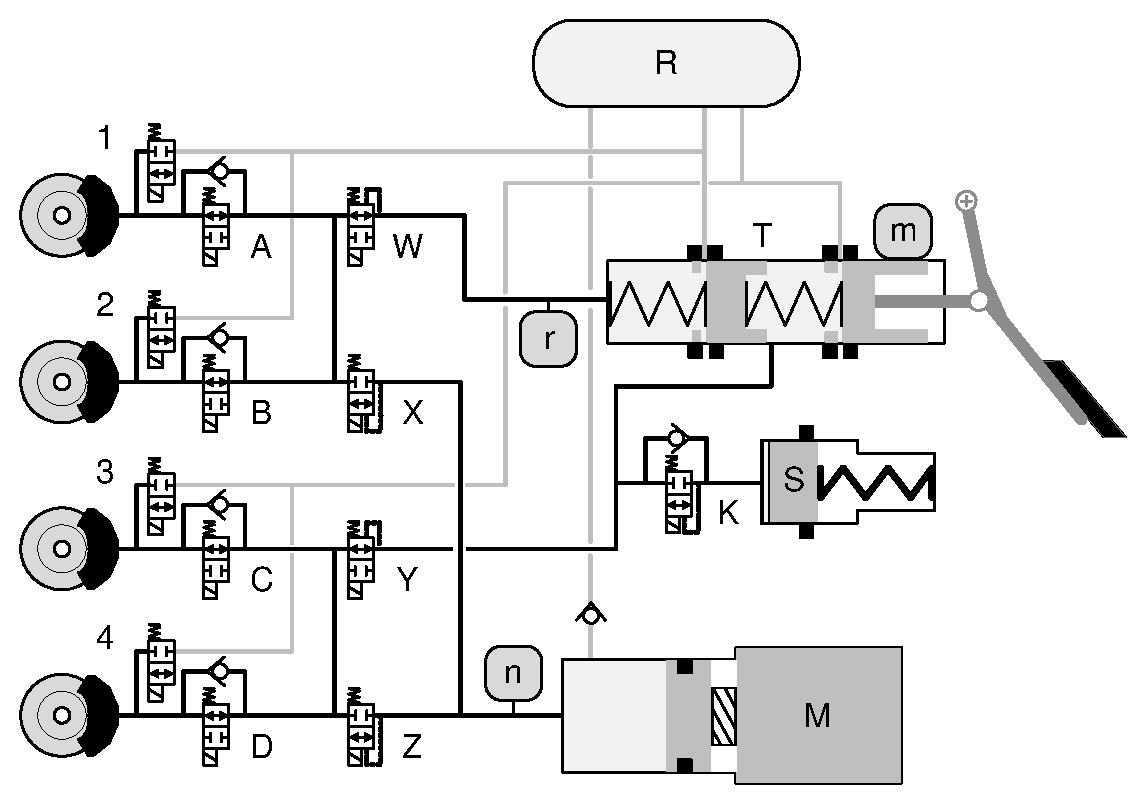
\includegraphics[width=1.\textwidth,clip, trim = 0cm 0cm 0cm 0cm]{2_EHB_Komponenten.eps}
 \caption[Elektrohydraulisches Bremssystem]{Elektrohydraulisches Bremssystem (EHB) mit Tandemhauptbremszylinders (THZ), elektrischem Zentraldruckaktor (M), Simulator (S), Ventilen (V$_{ij}$), Weg- (S$_{s}$) und Drucksensoren (S$_{pi}$) sowie Bremsflüssigkeitsreservoir (R); vgl.\cite{breuer20012bremsenhandbuch}}
 \label{fig:ehb_aufbau}
\end{figure} 


\subsubsection{Funktionsweise} \label{sec:ehb_funktionsweise}
Die Arbeitsweise der EHB wird aus Abb.\,\ref{fig:ehb_aufbau} ersichtlich, worin alle Ventile im stromlosen Zustand abgebildet sind. Den nehmen sie bei einem elektrischen Systemausfall ein, sodass die mechanische Rückfallebene wirksam wird. Betätigt der Fahrer dann das Bremspedal, so wird aus den beiden\footnote{Aus Redundanzgründen werden Bremssysteme immer in zwei getrennte Bremskreise aufgeteilt.} Kammern des Tandemhauptbremszylinders THZ durch die geöffneten Trennventile V$\!_{1c}$ und V$\!_{3c}$ und ABS-Einlassventile V$\!_{1i}$ -- V$_{4i}$ Öl zu den Bremsen gefördert, das infolge der geschlossenen ABS-Auslassventile V$\!_{1o}$ -- V$\!_{4o}$  und Trennventile V$\!_{2c}$ und V$\!_{4c}$ den Druck $p$ aufbaut. Aufgrund des geschlossenen Simulatorventils V$\!_s$ ist hierbei der Simulator S abgekoppelt, sodass die vom Fahrer auf das Pedal übertragene Betätigungsenergie ausschließlich dem behelfsmäßigen Verzögern der Räder dient. \\
Im Normalbetrieb sind V$\!_{1c}$ und V$\!_{3c}$ geschlossen sowie V$\!_s$, V$\!_{2c}$ und V$\!_{4c}$ geöffnet. Hierdurch gelangt das vom Fahrer verdrängte Volumen %des HBZ-Primärkreises 
ausschließlich in den Simulator, der das angestrebte Pedalgefühl realisiert. Über den Drucksensor S$_{p1}$ und den Wegsensor S$_s$ berechnet sich das Wunschbremsmoment des Fahrers und wird mit ggf.\ vorhandenen externen Vorgaben überlagert. Der abgeleitete Zielbremsdruck wird schließlich über den Zentraldruckaktor (M) unter Rückführung des Messwerts des Drucksensors S$_{p2}$ durch die offenen Ventile V$\!_{2c}$ und V$\!_{4c}$ in den beiden Bremskreisen eingeregelt. 
Über den sog.\ $C^\ast$-Wert\footnote{Verhältnis der in den Reibflächen entstehenden Umfangskraft zur aufgebrachten Spannkraft} der Bremse, die Bremskolbenfläche $A$ und den effektiven Bremsradius $r_\text{eff}$ berechnet sich das Bremsmoment zu
\begin{align*}
	M_B = C^\ast \cdot r_\text{eff}\cdot A \cdot p\;,
\end{align*}
worüber durch Auflösen der Sollbremsdruck an den Rädern bestimmt werden kann, der dann vom an den Fahrzeug-Bus angeschlossenen Bremssteuergerät eingeregelt wird.
Durch die vom Fahrer vollkommen entkoppelte Vorgabe von Bremsmomenten ist aus Fahrerassistenzsicht die mit brake-by-wire verknüpfte Flexibilität im vollen Umfang gegeben, 
ohne dass auf eine mechanische Rückfallebene verzichtet werden muss. \\
Zur radselektiven Bremsung, die für das ABS und ESP von so großer Bedeutung ist, können die Ventile V$\!_{1i}$ -- V$_{4i}$ und V$\!_{1o}$ -- V$_{4o}$ einzeln angesteuert werden, sodass der in den Bremsbacken anliegende Druck aufgebaut, gehalten oder abgelassen werden kann.

\subsection{Antrieb\index{Antrieb}} \label{sec:motorregelung}
% http://www.patent-de.com/20071122/DE19812485B4.html
% http://www.patent-de.com/19941110/DE69007902T2.html
Im Unterschied zu den Lenk- und Bremssystemen ist beim Verbrennungsmotor schon längst eine By-wire-Ansteuerung etabliert, das sog.\ \emph{E-Gas}\index{E-Gas} \cite{isermann2010mechatronische}. Das Gaspedal des Fahrers ist dabei nicht mehr mechanisch an den Motor gekoppelt, sondern besitzt einen Sensor zur Bestimmung des Pedalhubs, entsprechend dessen Messwert die Öffnung der elektronischen Drosselklappe eingestellt wird. Aufgrund des anhaltend hohen Stellenwerts des Verbrennungsmotors im Individualverkehr werden die für die Fahrerassistenz relevanten Aspekte der Motorregelung und der Getriebesteuerung nun nacheinander beleuchtet.  

\begin{figure}[h]
	\psfrag{Z}[cc][cc][1.0]{Z}
	\psfrag{E}[cc][cc][1.0]{E}
	\psfrag{n}[cc][cc][1.0]{S$_n$}
	\psfrag{D}[cc][cc][1.0]{D}
	\psfrag{p}[cc][cc][1.0]{S$_w$}
\centering
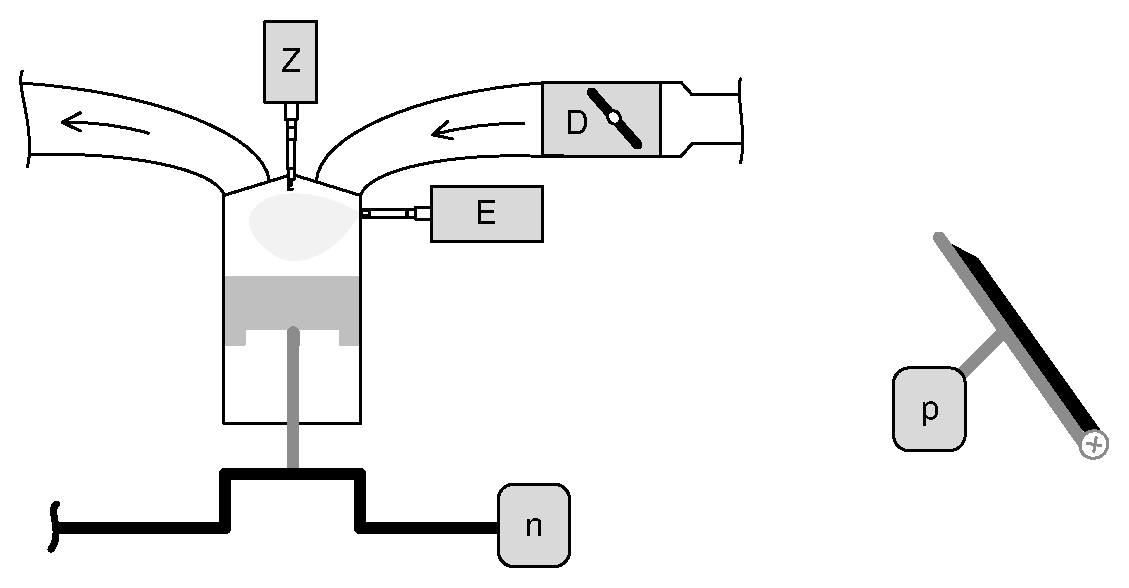
\includegraphics[width=.7\textwidth,clip, trim = 0cm 0cm 0cm 0cm]{2_Benzinmotor_Komponenten.eps}
 \caption[Vereinfachte Darstellung eines Saugeinspritzer-Motors]{Vereinfachte Darstellung eines Saugeinspritzer-Motors mit Pedalwertgeber (S$_w$), Motordrehzahl-Sensor (S$_n$), Drosselklappe (D), Einspritzventil (E) und Zündspule (Z); vgl. \cite{isermann2010mechatronische}}
 \label{fig:motor_aufbau}
\end{figure} 


\subsubsection{Funktionsweise der Motorregelung}
Bei einer modernen sog.\ \emph{drehmomentorientierten Regelung}\index{drehmomentorientierte Regelung} \cite{patentDE19812485B4, patentDE69007902T2} wird nicht einfach der ausgelesene Fahrerpedalwert $\alpha_d$ entsprechend eines simplen Kennfelds auf die Drosselklappenstellung $\alpha_e$ übertragen und damit eine mechanische Verbindung nachgeahmt. Vielmehr werden, analog zur Bremsmomentregelung in Abschn.\,\ref{sec:ehb_funktionsweise}, die Freiheitsgrade eines elektronischen Steuergeräts dazu genutzt, aus dem Fahrerpedalwert (erfasst durch S$_w$, s.\ Abb.\,\ref{fig:motor_aufbau}) zunächst ein Wunschantriebsmoment $M_d$ abzuleiten\footnote{Je nach Fahrmodus (\emph{Sport}, \emph{Eco} etc.) wird zwischen unterschiedlichen Pedalcharakteristiken umgeschalten.}, s.\ \abb{fig:motor_funktionsweise}. Nach Belieben kann es mit externen, \zB von der  Fahrerassistenz herrührenden Signalen $M_\text{FAS}$ zu einem Sollmoment überlagert werden. % und unter Berücksichtigung verschiedener Messgrößen (z.B.\ hauptsächlich die Drehzahl gemessen durch S$_n$) %über die Drosselklappe (D)  eingeregelt werden. 

\begin{figure}[h]
\newcommand{\smallsize}{.75}
	\psfrag{a}[cb][cb][1.0]{$\alpha_d$}
	\psfrag{b}[cr][cr][1.0]{$n$}
	\psfrag{c}[cb][cb][1.0]{$M_d$}
	\psfrag{d}[cb][cb][1.0]{$M_{id}$}
	\psfrag{e}[cb][cb][1.0]{$M_\text{FAS}$}
	\psfrag{f}[cb][cb][1.0]{$M_\text{ch}$}
	\psfrag{h}[cb][cb][1.0]{$M_\text{ig}$}
	\psfrag{j}[cb][cb][1.0]{$\alpha_e$}
	\psfrag{k}[cb][cb][1.0]{$\phi_\text{ig}$}
	\psfrag{l}[cb][cb][1.0]{$t_i$}
	\psfrag{0}[cc][cc][1.0]{Motor}
	\psfrag{1}[cc][cc][1.0]{{\parbox[c]{7cm}{\begin{center} Fahrer- \\ assistenz \end{center}}}}
	\psfrag{2}[cc][cc][\smallsize]{{\parbox[c]{7cm}{\begin{center} Wunschmom.- \\ generierung \end{center}}}}
	\psfrag{3}[cc][cc][\smallsize]{{\parbox[c]{7cm}{\begin{center} Verlustmom.- \\ kompensation \end{center}}}}
	\psfrag{4}[cc][cc][\smallsize]{{\parbox[c]{7cm}{\begin{center} Luftmassen- \\ regelung \end{center}}}}
	\psfrag{5}[cc][cc][\smallsize]{{\parbox[c]{7cm}{\begin{center} Zündwinkel- u.\ \\ Einspritz-Strg.\ \end{center}}}}
	\psfrag{6}[cc][cc][\smallsize]{{\parbox[c]{7cm}{\begin{center} Dynamische \\ Moment- \\ aufteilung \end{center}}}}
\centering
\includegraphics[width=1.\textwidth,clip, trim = 0cm 0cm 0cm 0cm]{2_Benzinmotor_Regelung.eps}
 \caption[Drehmomentorientierte Regelung eines Saugmotors]{Drehmomentorientierte Regelung eines Saugmotors mit dynamischer Aufteilung des gewünschten inneren Drehmoments in ein niederfrequentes Basisdrehmoment für die Luftfüllung $M_\text{ch}$ und ein hochfrequentes Zusatzmoment $M_\text{ig}$ für Zündwinkel und Einspritzdauer, vgl.\ \cite{isermann2010mechatronische}} % mit Pedalwert $\alpha_d$, Wunschantriebsmoment $M_d$, inneres Wunschmoment $M_{id}$, Basismoment $M_\text{ch}$, Zusatzmoment $M_\text{ig}$, Drosselklappenwinkel $\alpha_e$, Zündwinkel $\phi_\text{ig}$ und Einspritzdauer $t_i$}
 \label{fig:motor_funktionsweise}
\end{figure} 

Nach der anschließenden Verlustmomentkompensation der Motorsteuerung\index{Motorsteuerung}, die der inneren Verlustleistung des Motors Rechnung trägt, wird nun der große Vorteil eines Steuergeräts ausgespielt. Die stark verzögerte Reaktion des Motormoments auf Änderungen der Drosselklappe, die auf die Trägheit des angesaugten Luftstroms zurückzuführen ist, erweist sich nämlich als großer Nachteil für den Fahrer und vor allem für ein sicherheitskritisches Assistenzsystem wie eine Antriebs-Schlupf-Regelung (ASR). Einen unmittelbaren Einfluss auf das innere Motormoment besitzen hingegen die Zündung und Einspritzung, da sie kurbelwellensynchron arbeiten. Aus dem Grund erfolgt entsprechend \abb{fig:motor_funktionsweise} eine Aufteilung des gewünschten inneren Drehmoments  $M_{id}$ in ein niederfrequentes Basisdrehmoment $M_\text{ch}$ für die Luftfüllung, eingeregelt mittels Drosselklappenwinkel $\alpha_e$, und ein hochfrequentes Zusatzmoment $M_\text{ig}$, realisiert durch Veränderung des Zündwinkels $\phi_\text{ig}$ und der Einspritzdauer $t_i$ (s.\ Abb.\,\ref{fig:motor_funktionsweise}). Die jeweiligen Berechnungen basieren dabei auf der Invertierung des Drehmoment- bzw. Luftmassenmodells in Abhängigkeit verschiedener Messgrößen wie der Motordrehzahl $n$. \\
Auf Basis eines guten Motormodells ist es nun nicht nur möglich, vorgegebene Antriebsmomente umzusetzen, sondern auch das Schleppmoment (Motormoment bei $\alpha_d=0$) hinreichend genau zu schätzen, sodass es zum automatischen Verzögern im angeforderten Bremsmoment bereits berücksichtigt werden kann. Sowohl beim Soll- als auch Istwert des Antriebsmoments handelt es sich in modernen Fahrerassistenzarchitekturen bereits
%, wie auch schon bei den Bremsmomenten, 
um Radantriebsmomente, sodass die Getriebeübersetzung des aktuellen Gangs berücksichtigt ist. %Bei Automatikgetrieben erfolgt die Gangwahl nach sog.\ Schaltkennlinien, die im anschließenden Abschnitt erläutert werden.
%




\subsubsection{Funktionsweise der automatischen Getriebesteuerung\index{Getriebesteuerung}} %Differentialsteuerung
Aufgrund ihrer komfortsteigernden, effizienten und umweltschonenden Arbeitsweise sind Automatikgetriebe aus dem Antriebsstrang nicht mehr wegzudenken. Insbesondere bei der Realisierung von Komfortassistenzsystemen der Längsführung, namentlich das ACC, führen sie zu einer großen Entlastung, da andernfalls der Fahrer schalten muss.
Ohne ins Detail von dem aufwändigen elektro-mechanischen Aufbau und der Regelung einzelner Komponenten eines Automatikgetriebes zu gehen, soll das Automatikgetriebe auf seine aus Fahrerassistenzsicht wichtigsten Eigenschaften, definiert durch Momentübersetzung und Schaltpunkte, reduziert werden.

In Verbindung mit Motor und Differential legt das Automatikgetriebe über die Gangwahl das Antriebsmoment an den Reifen fest. Als Hauptkriterien stehen sich dabei das maximal entfaltbare Antriebsmoment und der möglichst geringe Verbrauch gegenüber \cite{gruhle2010steuerung}. Um den Kompromiss besser aufzulösen, werden dem Fahrer unterschiedliche Schaltprogramme (\zB \emph{Eco} und \emph{Sport}) angeboten. Davon unabhängig kann permanent über Kickdown die Maximalleistung des Motors abgefragt werden. \\
Die Gangwahl eines Schaltprogramms erfolgt über sog.\ Schaltkennlinien\index{Schaltkennlinie}, die einen bestimmten Gangwechsel (z.B.\ von 1 nach 2) in Abhängigkeit der Pedalstellung und der Geschwindigkeit auslösen, s.\ Abb.\,\ref{fig:getriebe}. Zur Vermeidung von Schaltpendeln unterscheidet sich die Kennlinie des Hoch- von der des Herunterschaltens, sodass eine Hysterese entsteht.
Zur Optimierung des Schaltvorgangs, welcher im Unterschied zum Handschalter unter Last erfolgt, wird neben dem Kupplungsdruck der jeweiligen Gänge auch eine Abschwächung des Motormoments angefordert \cite{gruhle2010steuerung}, s.\ \abschn{sec:motorregelung}.

\begin{figure}[h]
\newcommand{\smallsize}{.75}
	\psfrag{1}[cb][cb][\smallsize]{2-1}
	\psfrag{2}[cb][cb][\smallsize]{1-2}
	\psfrag{3}[cb][cb][\smallsize]{3-2}
	\psfrag{4}[cb][cb][\smallsize]{2-3}
	\psfrag{5}[cb][cb][\smallsize]{4-3}
	\psfrag{6}[cb][cb][\smallsize]{3-4}
	\psfrag{7}[cb][cb][\smallsize]{5-4}
	\psfrag{8}[cb][cb][\smallsize]{4-5}
	\psfrag{9}[cb][cb][\smallsize]{6-5}
	\psfrag{0}[cb][cb][\smallsize]{5-6}
	\psfrag{a}[cr][cr][\smallsize]{20}
	\psfrag{c}[cr][cr][\smallsize]{40}
	\psfrag{e}[cr][cr][\smallsize]{60}
	\psfrag{i}[cr][cr][\smallsize]{80}
	\psfrag{m}[cr][cr][\smallsize]{100}
	\psfrag{k}[cr][cr][1.]{KD}
	\psfrag{n}[ct][ct][\smallsize]{25}
	\psfrag{o}[ct][ct][\smallsize]{50}
	\psfrag{r}[ct][ct][\smallsize]{75}
	\psfrag{s}[ct][ct][\smallsize]{100}
	\psfrag{u}[ct][ct][\smallsize]{125}
	\psfrag{v}[ct][ct][\smallsize]{150}
	\psfrag{w}[ct][ct][\smallsize]{175}
	\psfrag{x}[ct][ct][\smallsize]{200}
	\psfrag{z}[ct][ct][\smallsize]{225}
	\psfrag{b}[ct][ct][1.0]{Geschwindigkeit / \unitfrac{km}{h}}
	\psfrag{y}[cb][cb][1.0]{Fahrpedalstellung / \%}
\centering
\includegraphics[width=1.0\textwidth,clip, trim = 0cm 0cm 0cm 0cm]{2_Getriebe_Schaltung.eps}
 \caption[Qualitativer Verlauf der Schaltkennlinien]{Qualitativer Verlauf der Schaltkennlinien eines 6-Gang-Automatikgetriebes \cite{gruhle2010steuerung}, Hochschalten in Schwarz, Herunterschalten in Grau, Kickdown (KD)}
 \label{fig:getriebe}
\end{figure} 


Für die Fahrerassistenz hat sich als Schnittstelle zum Antrieb, analog zum Radbremsmoment, das Gesamtantriebsmoment als Summe der angetriebenen Räder etabliert. Der damit verbundene Hauptvorteil liegt darin, dass aus Fahrerassistenzsicht kein Wissen über den Antriebsstrang vorhanden sein muss, da das Zusammenspiel aus Getriebe- und Motorsteuerung das Sollmoment bestmöglich umsetzt. 
Soll darüber hinaus die Antriebskraft unter den einzelnen Rädern umverteilt werden (es wird auch von \emph{torque vectoring} \cite{piyabongkarn2007use, fallah2012controller} gesprochen), so muss dies über ein sog.\ Sperrdifferential\index{Sperrdifferential}\footnote{Zur Unterscheidung beschreibt eine Differentialsperre eine hinzuschaltbare mechanische Verbindung, die keinerlei Drehzahlunterschied zwischen den Rädern zulässt.} erfolgen. Es bremst die Ausgleichsbewegung der einzelnen Räder und sorgt damit für eine, wenn auch verlustbehaftete Umverteilung der Antriebskraft. Insbesondere bei variierendem Fahrbahnuntergrund kann dadurch die Traktion deutlich verbessert werden.%, was genauer in \abschn{sec:torque_vectoring} erläutert wird.

Damit sind alle zur Realisierung aktiver Fahreingriffe verfügbaren Stellgrößen qualitativ beschrieben und es kann im nächsten Abschnitt auf die Systemeingangsgrößen eingegangen werden.




% Wie im eingangs genannten Stand der Technik beschrieben wird dabei aus dem Betätigungsgrad des Bedienelements des Fahrers unter Berücksichtigung wenigstens der Motordrehzahl ein vom Fahrer vorgegebener Sollmomentwert gebildet, der gegebenenfalls mit den von anderen Steuer- bzw. Regelsystemen gebildeten Momentwerten verglichen und ein Sollmomentwert ausgewählt wird, der zur Einstellung des Drehmoments der Brennkraftmaschine dient. Bezüglich der Einstellung der Luftzufuhr wird dabei, wie aus dem Stand der Technik bekannt, der Soll-Momentwert in einen Sollwert für die Zylinderfüllung umgewandelt, der wiederum in einen Sollwert für die Stellung der Drosselklappe umgewandelt wird. Zur Regelung des Ist-Moments auf das Sollmoment werden dann neben der Luftzufuhr in der aus der Stand der Technik bekannten Weise auch in die Zündwinkeleinstellung, die Kraftstoffzufuhr, etc. eingegriffen.


%Redundantes Signal für Last: Saugrohrdrucks bzw. des Luftmassenmessers Bei heutigen Steuersystemen werden wenigstens zwei Messeinrichtungen eingesetzt, beispielsweise ein Sensor zur Erfassung der Drosselklappenstellung und ein Sensor zur Erfassung der zuströmenden Luftmasse oder aber ein Sensor zur Erfassung des Saugrohrdrucks.
% http://www.patent-de.com/20071122/DE19812485B4.html



\section{Sensorik, Mess- und Schätzgrößen}
Sowohl die Trajektorienoptimierung als auch ein Großteil der unterlagerten Regler beruhen auf dem Prinzip der Zustandsrückführung (im Unterschied zur Ausgangsrückführung). Es verwundert in der Praxis daher nicht, dass das Leistungsvermögen des Gesamtsystems maßgeblich von der Qualität der Sensorik und Messgrößenaufbereitung bestimmt wird. Schließlich kann das Fahrzeug weitaus bessere Entscheidungen über die einzuschlagende Trajektorie treffen, wenn es genaue Kenntnis über seinen eigenen Fahrzustand und den anderer Verkehrsteilnehmer (Abstand, Bewegungsrichtung etc.) besitzt. Zugleich wird die Stabilisierungsebene durch ein latenzarmes Messsignal dazu befähigt, auf Störungen schnell zu reagieren, um eine optimierte Trajektorie möglichst genau umzusetzen. Im Folgenden wird daher die den Assistenzfunktionen im Fahrzeug zur Verfügung stehende Information beschrieben und ein kurzer Einblick in die für sie wesentlichen Aspekte der Entstehung gegeben. Die Einteilung in Eigenfahrzeug- (im Folgenden mit Ego bezeichnet) und Fahrzeugumfeld-bezogene Information erweist sich hierbei als zweckmäßig.

%Grundsätzlich kann über die Mess- und Schätzgrößen in eigenfahrzeugbezogene und umweltbezogene unterschieden werden
% correvit
\label{sec:sensoren} % Lenkwinkelsensor

\subsection{Fahrzustandserfassung\index{Fahrzustandserfassung}} \label{sec:eigenfahrzustandserfassung}
So wie der menschliche Fahrer über seine vestibuläre\footnote{Das Gleichgewichtsorgan wird auch als Vestibularapparat bezeichnet.} und visuelle Wahrnehmung muss ein Assistenzsystem über die Fahrzeugsensorik den aktuellen Fahrzustand erfassen und das möglichst präzise. Hierzu steht ihm insbesondere die Inertialsensorik zur Verfügung, welche im Fahrzeug als sog.\ \emph{Sensorcluster} die Beschleunigungen und Drehraten in den für die Fahrdynamik relevanten Richtungen misst. Darüber hinaus sind mit der gewonnenen Messinformation unter Einbezug weiterer Messgrößen die Fahrzeuglängs- und Quergeschwindigkeit zu schätzen, da sie aus Kostengründen in Serienfahrzeugen nicht direkt gemessen werden.

\subsubsection{Funktionsweise Sensorcluster\cite{Sensorcluster}}
Während für Stabilitätsprogramme wie das ESP neben der Quer- und Längsbeschleunigung die Drehrate um die Fahrzeughochachse als Messgröße ausreichend ist, erfordern automatische Überrollschutzsysteme von Fahrzeugen mit erhöhtem Schwerpunkt zusätzlich die Erfassung der Drehrate um die Fahrzeugquer- und -längsachse. Das sog.\ \emph{Sensorcluster} umfasst nun zentral die entsprechend ihrer Messachsen %der jeweiligen Messgröße 
ausgerichteten Beschleunigungs-\index{Beschleunigungssensor} und Drehratensensoren \index{Drehratensensor} und stellt deren Messsignale auf dem Fahrzeug-Bus den Steuergeräten zur Verfügung \cite{reif2010sensoren}. 
\begin{figure}[ht]
\newcommand{\smallsize}{.75}
	\psfrag{f}[cl][cl][1.0]{$F_a$}
	\psfrag{b}[cr][cr][1.0]{Auslenkung}
	\psfrag{m}[cc][cc][1.0]{$m$}
	\psfrag{a}[cr][cr][1.0]{$a$}
\centering
\includegraphics[width=.5\textwidth,clip, trim = 0cm 0cm 0cm 0cm]{2_querbeschleunigungssensor.eps}
 \caption[Funktionsweise eines Beschleunigungssensors]{Funktionsweise eines mikro-elektro-mechanischen Beschleunigungssensors: Aufgrund der zu messenden Beschleunigung $a$ erfährt die Masse $m$ eine Messkraft $F_a$, die zu einer zur Beschleunigung proportionalen Auslenkung führt \cite{reif2010sensoren}.}
 \label{fig:querbeschleunigungssensor}
\end{figure}
%
Im Automobilbereich haben sich sog.\ \emph{mikro-elektro-mechanische} (MEM) Beschleunigungs- und Drehratensensoren etabliert, die aus filigranen mechanischen Silizium-Strukturen und elektronischen Auswerteeinheiten bestehen. Zwar unterscheiden sich die Sensoren im Aufbau von Hersteller zu Hersteller, in ihrer grundsätzlichen Funktionsweise decken sie sich jedoch. Zur Erklärung sei \abb{fig:querbeschleunigungssensor} betrachtet, in der 
das Messprinzip der Querbeschleunigung verdeutlicht wird. Die elastisch gelagerte Masse $m$ erfährt bei einer Beschleunigung $a$ die Trägheitskraft $F_a$, was zu einer kapazitiv messbaren Auslenkung führt, sodass über die Federsteifigkeit und Masse auf $a$ geschlossen werden kann. Alternativ wird die Masse durch eine schnelle Lageregelung in ihrer Position gehalten, womit die erforderliche Kompensationskraft der Regelung der Trägheitskraft entspricht. Das erhöht den Messbereich (Amplitude und Grenzfrequenz), da die Masse sehr nahe am Nullpunkt der Auslenkung bleibt und somit ein lineares Systemverhalten gewährleistet ist.  \\
%

Die Messung der Drehrate erfolgt ebenfalls unter Ausnutzung von Trägheitseffekten. Allerdings werden hierzu zwei miteinander verbundene Masseschwinger angeregt, sodass sie gegensätzlich in ihrer gemeinsamen Resonanzfrequenz ($\approx \unit[1]{kHz}$) schwingen, s.\ \abb{fig:stimmgabe_gyro}. Bei einer Drehbewegung $\Omega$ senkrecht zur Oszillationsbewegung erfahren dann die Massen die Coriolis-Kraft, was eine Schwingung aus der Ebene heraus mit einer Amplitude proportional zur Gierrate induziert, die wiederum elektrostatisch gemessen werden kann \cite{reif2010sensoren}.
\begin{figure}[h]
\newcommand{\smallsize}{.75}
	\psfrag{2}[cc][cc][1.0]{$\Omega$}
	\psfrag{a}[ct][ct][1.0]{Anregung}
	\psfrag{c}[cl][cl][1.0]{Coriolis-Kraft}
	\psfrag{t}[ct][ct][1.0]{$t$}
	\psfrag{b}[cl][cl][1.0]{\parbox[r]{1.5cm}{Induzierte \\ Schwingung}}
\centering
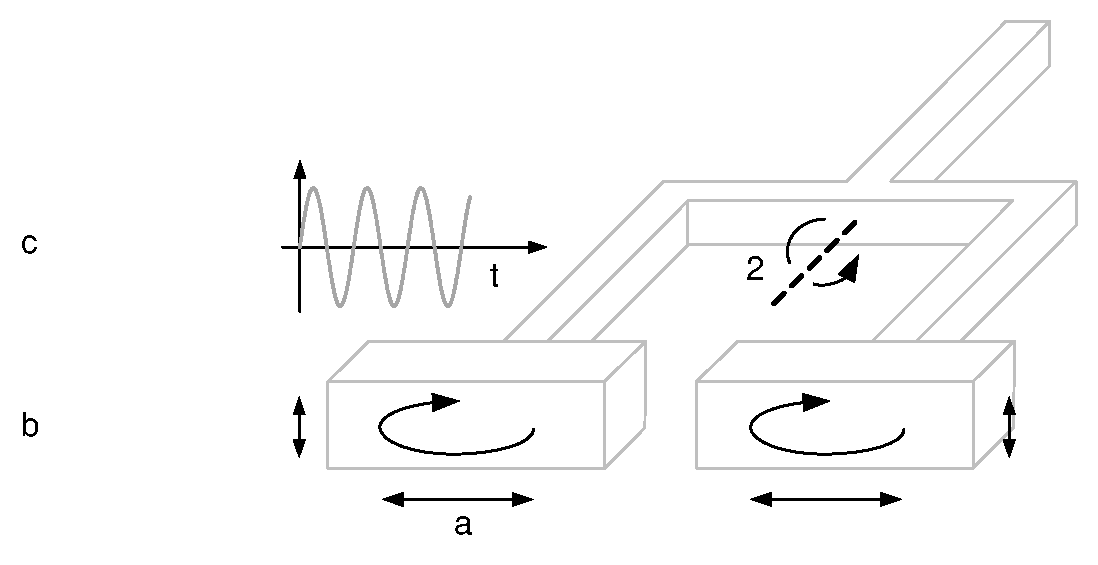
\includegraphics[width=.75\textwidth,clip, trim = 0cm 0cm 0cm 0cm]{2_stimmgabe_gyro.eps}
 \caption[Funktionsweise eines Drehratensensors]{Funktionsweise eines mikro-elektro-mechanischen Drehratensensors: Durch die Coriolis-Kraft erfahren die zur Oszillation angeregten Massen eine der Drehrate $\Omega$ proportionale Querauslenkung \cite{reif2010sensoren}.}
 \label{fig:stimmgabe_gyro}
\end{figure}


\subsubsection{Geschwindigkeits-\index{Geschwindigkeitsschätzung} und Schwimmwinkeschätzung\index{Schwimmwinkeschätzung}} \label{sec:beta_v} % not my business -> Literaturverweis
Da die Dynamik des Fahrzeugs grundlegend von seiner Geschwindigkeit beeinflusst wird, erfordern die meisten Assistenzfunktionen ein genaues Längsgeschwindigkeitssignal $v_x(t)$. Gerade aber im fahrphysikalischen Grenzbereich weisen die Reifen erheblichen Schlupf\footnote{Die normierte Geschwindigkeitsdifferenz zwischen Fahrbahn und Reifen in der Kontaktfläche wird als Schlupf bezeichnet.} auf, sodass von den Raddrehzahlsensoren (s.\ \cite{reif2010sensoren}) nur unzureichend auf die Fahrzeuggeschwindigkeit geschlossen werden kann. Ebenso verhält es sich bei der Fahrzeugquergeschwindigkeit $v_y(t)$, die bei einem schleudernden Fahrzeug ganz erhebliche Werte annehmen kann. Wenn auch im Rennsport und Erprobungsbetrieb Geschwindigkeitsmesssysteme über Grund verwendet werden (optisch \cite{horn2006zweidimensionale} oder mittels hoch genauer, GPS-gekoppelter Inertialsensorik \cite{ryu2004integrating}), so verbietet sich aus Kostengründen deren Einsatz im Serienfahrzeug. Da aufgrund des Messrauschens bei einer reinen Aufintegration der Drehraten- und Beschleunigungssignale die Genauigkeit rapide abnimmt, müssen die Geschwindigkeiten geschätzt werden, was der Zuhilfenahme von Fahrzeugmodellen bedarf. \\
Die Längsgeschwindigkeitsschätzung erfolgt so, dass auch während einer ABS-Bremsung einzelne Räder gezielt "`unterbremst"' werden und dadurch nach kurzer Zeit stabil laufen. Aus der sich dann ergebenden Raddrehzahl kann über das anliegende Radbremsmoment (s.\ \abschn{sec:ehb_funktionsweise}) und die Reifencharakteristik auf die Geschwindigkeit über Grund geschlossen werden. Unter Berücksichtigung des Lenkwinkels und der Giergeschwindigkeit wird dann die Umrechnung in den Schwerpunkt vorgenommen. Über die Differentialgleichung der Längsgeschwindigkeit erfolgt die Sensorfusion mittels erweitertem Kalman-Filter\index{Kalman-Filter} \cite{kalman1960new}, s.\, \cite{BHB2012_vanZanten_bremsanlage}. \\
Ähnlich verhält es sich bei der Querbewegung, wobei i.\,Allg.\ anstelle von $v_y$ die zum Fahrzeug relative Bewegungsrichtung
\begin{align*}
	\beta = \arctan(v_y/v_x)\;,
\end{align*}
der sog.\ \emph{Schwimmwinkel}\index{Schwimmwinkel}, als Zustandsgröße herangezogen wird, s.\ \abb{fig:fahrzeugbewegung}. Analog zur Längsgeschwindigkeitsschätzung wird über die Differentialgleichung der Querbewegung der Schwimmwinkel mittels erweitertem Kalman-Filter aus der Fahrzeugdrehrate um die Hochachse, der Querbeschleunigung und dem Lenkwinkel geschätzt \cite{tno2007_stateestimator, BHB2012_vanZanten_bremsanlage, Konig2008}.
\begin{figure}[h]
\centering
\newcommand{\smallsize}{.85}
	\psfrag{x}[tc][tc][1.0]{$x_1$}
	\psfrag{y}[rc][rc][1.0]{$x_2$}
	\psfrag{m}[tl][tl][1.0]{$v_y$}
	\psfrag{n}[tl][tl][1.0]{$v_x$}
	\psfrag{b}[cc][cc][1.0]{$\beta$}
	\psfrag{p}[cc][cc][1.0]{$\psi$}
	\psfrag{v}[rb][rb][1.0]{$v$}
	\psfrag{t}[lb][lb][1.0]{$\theta$}
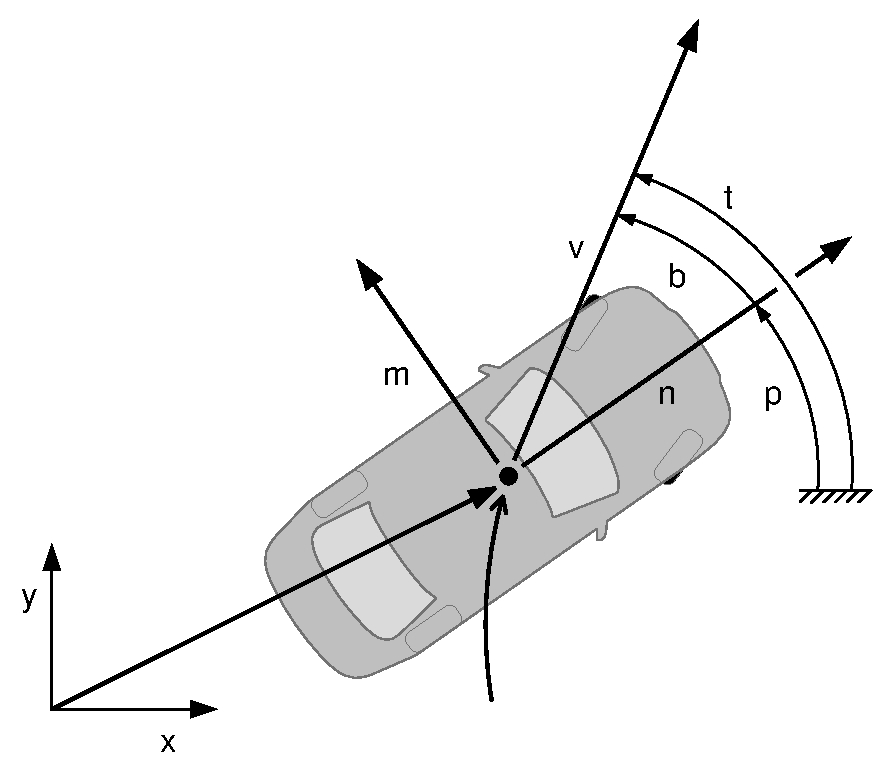
\includegraphics[width=.55\textwidth,clip, trim = 0cm 0cm 0cm 0cm]{2_Kinematik.eps}
 \caption[Bewegungskinematik des Fahrzeugs]{Bewegungskinematik des Fahrzeugs innerhalb eines ortsfesten Koordinatensystems $[x_1, x_2]$}
 \label{fig:fahrzeugbewegung}
\end{figure} 



\subsection{Eigenlokalisierung\index{Eigenlokalisierung}}
Wie bereits 1986 praktisch nachgewiesen wurde \cite{dickmans1989sod}, kann bei vorhandenen Fahrbahnmarkierungen ein Fahrzeug der Spur selbständig folgen, und das ohne jegliche Art einer globalen Eigenlokalisierung. Schließlich reicht es aus, wenn regelmäßig die Fahrzeugrelativposition und -ausrichtung zu den Spurmarkierungen aus einer Kamera bestimmt und Abweichungen von der so bestimmten Fahrbahnmitte über Lenkbefehle minimiert werden\footnote{Eine Alternative stellt das Einlassen von stromdurchflossenen Drähten oder das Einschlagen von Magneten in die Fahrbahn dar, s.\ beispielsweise\ \cite{markgraf2002autonomes, tan1999development}.}. Die Robotik verwendet hierfür auch den Begriff \emph{visual servoing}\index{visual servoing} \cite{allen1991real}, da Regelabweichungen direkt aus dem Sensor bezogen werden. Dasselbe Prinzip findet in Fahrzeuglängsrichtung in der serienmäßig verfügbaren Komfortfunktion ACC ebenfalls Anwendung \cite{venhovens2000stop}, die mit dem nach vorne gerichteten Radar die Relativbewegung zum Vorderfahrzeug vermisst und einen vorgegebenen Abstand automatisch über Brems- und Motoreingriffe einregelt. Problematisch wird es allerdings, wenn bereits für kurze Zeit die Regelgrößen nicht verfügbar sind (z.B.\ kurzzeitiges Gegenlicht beim Spurhalten), da dann aufgrund der fehlenden Messgröße vom Regler keine Stellgröße berechnet werden kann. \\
Für einige Anwendungen im Fahrzeug verbietet sich gar funktionsbedingt das Prinzip des visual servoing. So kann zwar ein Einparkassistent durch einen  seitlichen Sensor die Größe und Relativposition einer Parklücke bei der Vorbeifahrt gut bestimmen, während des Manövers ist diese Information aber aufgrund der veränderten Sensorperspektive nicht verfügbar, sodass die Position relativ zur Parklücke anderweitig geschätzt werden muss. Ähnlich verhält es sich beim Ausweichen, während dessen eine nach vorne gerichtete Sensorik aufgrund der starken Drehbewegung um die Fahrzeughochachse (das sog.\ Gieren) kurz nach dem Auslenken das Hindernis verliert. Die übergeordnete Fragestellung ist in den Situationen demnach, wohin sich das Hindernis oder die Spur relativ zum Fahrzeug innerhalb des letzten Zeitabschnitts bewegt haben. Um das zu beantworten, bietet es sich an, mit Hilfe der geschätzten Egobewegung und fahrzeugfester Umfeldsensorik die Hindernisbewegung über Grund zu ermitteln, über der Zeit zu verfolgen \cite{maurer2005fahrerassistenzsysteme} und, falls erforderlich, zu prädizieren. Wenn auch noch die geschätzte Egobewegung aufintegriert wird, dann kann trotz kurzzeitig verdecktem Hindernis auf dessen Relativposition zum Fahrzeug geschlossen werden. Die Aufintegration wird auch als Koppelnavigation\index{Koppelnavigation} bezeichnet und in \abschn{sec:koppelnavi} erläutert. \\
%eine Aufteilung der Relativbewegung in Fahrzeugeigen- und Hindernisbewegung (letztere trivial bei statischen Hindernissen) über Grund an, eine Herangehensweise, die sich nicht nur bei hochautomatisierten Fahrzeugen (s.\ \zB \cite{jfr2008}) bewährt hat, weil hierdurch ganz allgemein die Hindernisbewegung besser gefiltert werden kann\footnote{Wird auch als Tracking bezeichnet \cite{todo}}. 
%An dieser Stelle sei bereits angemerkt, dass e
Sollen hingegen global referenzierte Informationen wie Straßenkarten herangezogen werden, dann ist zusätzlich eine globale Positionsbestimmung (beispielsweise über GPS) erforderlich, was in \abschn{sec:globalelok} beleuchtet wird. 
%Da die Hindernisbewegung im Rahmen der Situationsprädiktion noch genauer in Abschn.\,\ref{sec:praediction} beleuchtet wird, soll an dieser Stelle die Bestimmung der Eigenbewegung und Positionierung ausgeführt werden.

\subsubsection{Lokale Bestimmung von Egoposition und -ausrichtung} \label{sec:koppelnavi}
Ungeachtet der Ursache einer Bewegung beschäftigt sich die Kinematik mit der Bewegung von Körpern im Raum und ist damit Grundlage der Fahrzeugbewegung. Zur Beschreibung der rotatorischen und translatorischen Bewegung in der Ebene reicht die Geschwindigkeit $v$ eines fahrzeugfesten Referenzpunkts über Grund sowie dessen aktuelle Bewegungsrichtung $\theta$ (Kursrichtung\index{Kursrichtung}) und die Fahrzeugorientierung\index{Fahrzeugorientierung} $\psi$ aus, wobei  $\theta$ und $\psi$ relativ zu einem ortsfesten Koordinatensystem definiert werden. Wie anhand von Abb.\,\ref{fig:fahrzeugbewegung} nachvollzogen werden kann, genügt die Position $[x_1, x_2]$ dann der Differentialgleichung
\begin{align*}
	\dot x_1 &= v \cos\theta \\
	\dot x_2 &= v \sin\theta\,.
\end{align*}
Der Kurswinkel wiederum lässt sich aufteilen in
%In den meisten Anwendungen fehlt allerdings eine absolute Orientierungsreferenz, sodass $\theta$ und $\psi$ unbekannt sind und geschätzt werden müssen\footnote{Dasselbe gilt für $v$ im Fall von hochdynamischen Fahrmanövern, bei denen aufgrund des starken Schlupfs die Raddrehzahlen nicht unmittelbar die Fahrzeugbewegung spiegeln, s.\ Abschn.\,\ref{todo:ABS}.}. Hierzu bietet sich die Aufteilung des Kurswinkels in
\begin{align*}
	\theta = \psi + \beta\, ,
\end{align*}
wobei $\beta$ die Bewegungsrichtung relativ zum Fahrzeug beschreibt, s.\ Abb.\,\ref{fig:fahrzeugbewegung}. Falls der Bezugspunkt im Fahrzeugschwerpunkt liegt, wird $\beta$ auch als Schwimmwinkel\index{Schwimmwinkel} bezeichnet, s. \abschn{sec:beta_v}. \\
%
%  Dieser kann entweder optisch gemessen (s.\ Correvit, Visual Odometrie) oder unter Einbezug der Fahrphysik geschätzt werden (s.\ Abschn.\ref{sec:}). 
Ist auf eine direkte Bestimmung der Fahrzeugausrichtung, etwa durch einen Kompass, zu verzichten, so muss zusätzlich die Fahrzeuggierrate\index{Gierrate} $r=\dot \psi$ gemessen oder geschätzt\footnote{Bei langsamer Fahrt liefert das kinematische Einspurmodell eine sehr genaue Schätzung für die Gierrate, s.\ \abschn{sec:anhaengerdynamik}.} werden, und es ergibt sich insgesamt die Fahrzeugbewegung zu
\begin{align*}
	\dot x_1 &= v \cos(\psi + \beta) \\
	\dot x_2 &= v \sin(\psi + \beta) \\
  \dot   \psi &= r \,.
\end{align*}
Die sog.\ Koppelnavigation\index{Koppelnavigation} (engl.\ \emph{dead reckoning}) stellt nun nichts weiter dar, als die Aufintegration der drei\footnote{In der Schifffahrt, dem Ursprung der Koppelnavigation, entfällt die letzte Gleichung, da dort ein Kompass verwendet werden kann, dessen Einsatz sich aufgrund von Feldstörungen im Fahrzeug verbietet. Die relative Fahrtrichtung $\beta$ über Grund wird durch die sog.\ \emph{Beschickung} berücksichtigt, welche der Versetzung durch Strömung und Wind Rechnung trägt \cite{dreyer_sks}.} Differentialgleichungen, was problemlos numerisch erfolgen kann. Da die Raddrehzahlen in die Geschwindigkeit eingehen, wird in dem Zusammenhang in der Fahrerassistenz häufig auch der Ausdruck \emph{Odometrie\index{Odometrie}}\footnote{Positionsbestimmung anhand der zurückgelegten Wegstrecke; bei Schätzung der Fahrzeugbewegung aus der Kamera wird gar von \emph{visual odometry} gesprochen \cite{lategahn2012motion}.} gebraucht.

Bei der Aufintegration akkumulieren sich allerdings über der Zeit das Sensorrauschen von $r$, der Schätzfehler in der Geschwindigkeit $v$ und dem Schwimmwinkel $\beta$ sowie die numerischen Ungenauigkeiten auf. Dieses als \emph{Drift}\index{Drift} bezeichnete Phänomen ist in Abb.\,\ref{fig:Odo_drift} aus der Sicht einer Fahrerassistenzfunktion verdeutlicht. Dabei wird die Ursprungsposition (weißes Fahrzeug) mit der aktuellen Fahrzeugposition (graues Fahrzeug) durch die tatsächlich gefahrene Trajektorie (schwarze Linie) verbunden. Aufgrund der mit der Koppelnavigation verbundenen Fehler verschlechtert sich die Positions- und Orientierungsschätzung je länger die Fahrt andauert, sodass die vermeintlich gefahrene Trajektorie (grau) immer stärker von der tatsächlichen abweicht. Genauer gesagt: Kehrt das Fahrzeug wieder zum mutmaßlichen Ursprung der Trajektorie zurück, so weicht es dann um den aktuellen Drift in seiner Position und Ausrichtung von den eigentlichen Werten ab. \\
Für viele Anwendungen stellt der auf den Drift zurückzuführende Fehler jedoch kein Problem dar, weil sich die meisten Assistenzfunktionen lediglich auf Zeitpunkte zurückbeziehen, die nicht weit in der Vergangenheit liegen (s.\ kleine und große Ellipsen in Abb.\,\ref{fig:Odo_drift}).

\begin{figure}[h]
\newcommand{\smallsize}{.85}
\psfrag{N}[rc][rc][\smallsize]{Nord}
\psfrag{O}[tr][tr][\smallsize]{Ost}
\psfrag{d}[tr][tr][\smallsize]{Drift}
\psfrag{m}[br][br][1.0]{$T_\text{glob}(0)$}
\psfrag{n}[tl][tl][1.0]{$T_\text{glob}(t)$}
\psfrag{s}[cl][cl][\smallsize]{Ortsfestes KOS}
\psfrag{x}[cr][cr][\smallsize]{vermeintliche Trajektorie}
\psfrag{z}[cl][cl][\smallsize]{tatsächliche Trajektorie}
	\psfrag{1}[tl][tl][\smallsize]{\parbox[c]{7cm}{\begin{flushleft} großer \\ Fehler \end{flushleft}}}
		\psfrag{0}[bc][bc][\smallsize]{\parbox[c]{7cm}{\begin{center} kleiner \\ Fehler \end{center}}}
\psfrag{q}[tr][tr][\smallsize]{\parbox[c]{1cm}{\begin{centering} Fahrzeugfestes \\ KOS \end{centering}}}
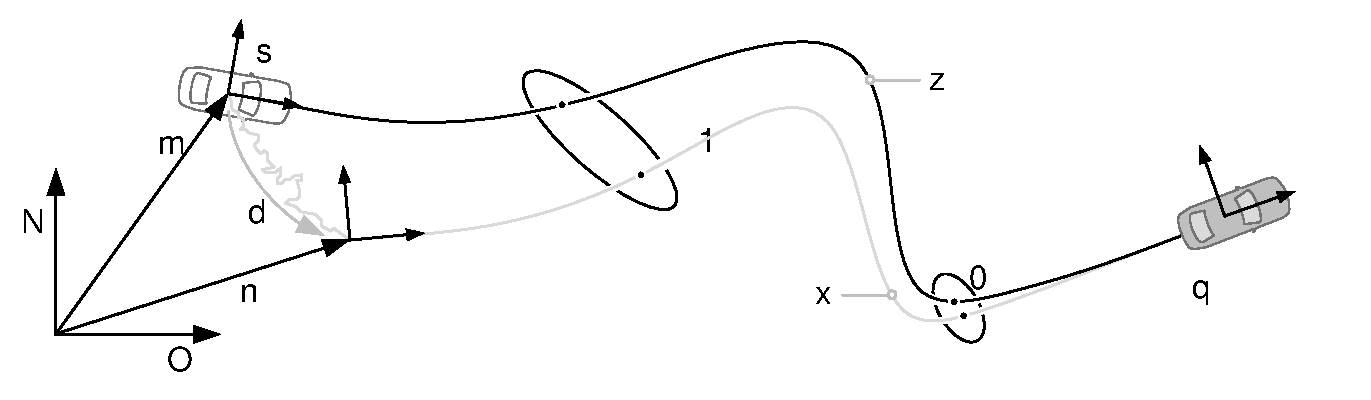
\includegraphics[width=1.\textwidth,clip, trim = 0cm 0cm 0cm 0cm]{2_koppelnavi_drift.eps}
 \caption[Mit Drift verbundene ortsfeste Koordinaten]{Veranschaulichung der mit Drift verbundenen ortsfesten Koordinaten}
 \label{fig:Odo_drift}
\end{figure} 

 

\subsubsection{Globale Bestimmung von Egoposition und -ausrichtung} \label{sec:globalelok}
Für die Umsetzung moderner Assistenzfunktionen der Führungsebene sind detaillierte Umfeldinformationen\index{Umfeldinformationen} wie zukünftiger Straßenverlauf und Vorfahrtsregelungen vonnöten, die durch aktuelle Umfeldsensorik und deren Auswertealgorithmik nur unzureichend zur Verfügung gestellt werden können. Insbesondere die im Rahmen der DARPA Urban Challenge\index{DARPA Urban Challenge} entstandenen Arbeiten  \cite{urmson2008adu, montemerlo2008junior, bacha2008odin, jfr2008} belegen jedoch, dass ein solches Defizit größtenteils durch global-referenzierte Daten ausgeglichen werden kann. Maßgeblich für die Verlässlichkeit der Karteninformation\index{Karteninformation} ist dabei neben der Genauigkeit vor allem deren Aktualität. Während es ausreichend sein kann, die Straßeninformation außerhalb von Baustellen nur einmal am Tag auf dem Fahrzeug zu aktualisieren, erfordern dynamische Gefahrenquellen, wie liegen gebliebene Fahrzeuge oder gar an eine Kreuzung herannahende Fahrradfahrer, eine permanente, latenzarme Informationsübertragung mittels Fahrzeug-zu-Fahrzeug- oder Fahrzeug-zu-Infrastruktur-Kommunikation (Car-to-X, kurz C2X), s.\ beispielsweise \citeltex{eichhorn2013Maneuverprediction, Werling_Vernetzung2012}. \\
Unabhängig von der Aktualisierungsrate ist es zur Nutzung der übermittelten Karteninformation wichtig zu wissen, an welcher Stelle der Karte und mit welcher Ausrichtung sich das Egofahrzeug befindet, was wiederum eine hinreichend genaue Bestimmung der globalen Fahrzeugposition und -ausrichtung erfordert. \\
Eine Möglichkeit hierfür stellt die Verwendung von GPS (Global Positioning System\index{Global Positioning System}) dar, das  
schon heute die Unterstützung des Fahrers durch Navigationsgeräte ermöglicht. Die Qualität und Verfügbarkeit von GPS unterliegt insbesondere im städtischen Bereich jedoch starken Schwankungen, sodass nach Alternativen gesucht wird 
\cite{pink2010bildbasierte, geiger2012we,levinson2010robust}. Für Hilfestellung sorgt hierbei die Robotik mit einer Vielzahl 
von Lokalisierungsverfahren \cite{borenstein1997}, die mittels Laserscannern \citeltex{Levinson2011} und Videokameras \cite{lategahn2013mapping} die Umgebung 
erfassen und geeignete Landmarken\index{Landmarke} bestimmen. Sind deren Positionen ebenfalls in einer Karte verzeichnet, kann über Triangulation auf die Roboterposition und -ausrichtung geschlossen\footnote{Erfolgt die Kartenerstellung auf Basis der gleichzeitigen Schätzung der Position aus Umfelddaten, so wird von \emph{simultaneous localization and mapping \index{simultaneous localization and mapping}} (SLAM) gesprochen, s.\ beispielweise \cite{Thrun2005, geiger2012we, kohlhepp2007elastic}.} und das Ergebnis mit der lokalen Positionsschätzung des vorherigen Abschnitts fusioniert werden. Angesichts der vermehrt eingesetzten Umfeldsensoren im Fahrzeug wird eine solche landmarkenbasierte Lokalisierung auch für die Fahrerassistenz interessant, sodass auf serientaugliche Alternativen zum GPS in den nächsten Jahren zu hoffen ist.

In der Funktionsarchitektur ist grundsätzlich bei der Wahl der Koordinatenursprünge darauf zu achten, dass sich Korrektursprünge der globalen Eigenlokalisierung nur auf Module auswirken, die auch wirklich auf eine absolute Position und Ausrichtung angewiesen sind. Eine saubere Trennung zwischen lokalen und globalen Koordinatensystemen, wie sie in \ref{app:kos} vorgeschlagen wird, ist daher unabdingbar.




\subsection{Fahrzeugumfeld-Modellierung und -Prädiktion}
Während für Assistenzsysteme der Stabilisierungsebene wie ESP die Schätzung des eigenen Fahrzeugzustands ausreicht (s.\ Abschn.\,\ref{sec:eigenfahrzustandserfassung}), so erfordert die Realisierung von Komfort- und Sicherheitsfunktionen der Führungsebene noch zusätzlich die Erfassung des Fahrzeugumfelds. Bereits heute ist eine Fülle von Umfeldsensorik im Serieneinsatz, namentlich Video\index{Video}, Radar\index{Radar}, Lidar\index{Lidar} und Ultraschall\index{Ultraschall}, deren jeweilige Messinformationen aufgrund unterschiedlicher Genauigkeiten und Erfassungsbereiche fusioniert werden. Angesichts der steigenden Funktionsanzahl im Fahrzeug ist es hierbei jedoch erstrebenswert, von einer funktionsspezifischen Sensordatenverarbeitung abzukommen, wie sie in der Serie aktuell gang und gäbe ist, und stattdessen die Messinformation zu einem generellen Abbild der Verkehrsszene zu fusionieren. Es kann dann als sog.\ \emph{Umfeldmodell\index{Umfeldmodell}} \cite{mahlisch2009filtersynthese} den verschiedenen Assistenzfunktionen zentral bereitgestellt werden. \\
Die Fahrzeugumfeld-Erfassung stellt allerdings eines der umfangreichsten Kapitel der Fahrerassistenz dar, sodass an dieser Stelle nur auf deren grundsätzlichen Aufbau und die für die Führungsebene wichtigsten Aspekte eingegangen werden kann. Zu letzteren zählen vor allem die Repräsentationsform der Hindernisse und der geschätzten Zustände einschließlich Unsicherheiten. %, da das Umfeldmodell der Manöverplanung als wichtige Schnittstelle dient. 
Welche Einzelschritte erforderlich sind, um von der zu jedem Messzeitpunkt erfassten Rohsensordateninformation zu einer Zustandsschätzung und Prädiktion der Umfeldobjekte zu gelangen, wird nun kurz skizziert. \\

\subsubsection{Mehrobjektverfolgung\index{Mehrobjektverfolgung}}
Nahezu alle bekannten Verfahren der \emph{Mehrobjektverfolgung} entsprechen der in \abb{fig:Klassische_Systemarchitektur_Tracking} dargestellten Systemarchitektur \cite{mahlisch2009filtersynthese}. In ihr werden im ersten Schritt die Rohdaten der Umfeldsensorik (Kamerabild \cite{dang2007kontinuierliche}, Lidar-Punktewolke \cite{moosmann2012interlacing}, Radar-Echo \cite{Diewald2013} etc.) auf Merkmale untersucht, die für die jeweilig zu erfassende Hindernisklasse (z.B. Fahrzeug, Fußgänger) sprechen. Das Ergebnis dieser \emph{Objektdetektion} ist eine Liste individuell erkannter Objekte, die im anschließenden Schritt der \emph{Objektassoziation} den bereits aus vorangegangenen Messungen verfolgten Hindernissen zugeordnet werden müssen.
Die Bewegungsschätzung eines jeden Objekts erfolgt anschließend unter Verwendung eines \emph{Zustandsfilters}, in dessen sog.\ Filterinnovation die von der Assoziation dem Objekt zugeordneten Messungen eingehen. Hierbei ist die Bewegung des Eigenfahrzeugs, s.\ \abschn{sec:eigenfahrzustandserfassung}, zu berücksichtigen.
\begin{figure}[h]
\newcommand{\smallsize}{.5}
	\psfrag{a}[cc][cc][1.0]{Objektdetektion}
	\psfrag{c}[cc][cc][1.0]{Objektassoziationen}
	\psfrag{e}[cc][cc][1.0]{Zustandsfilterung}
	\psfrag{m}[cc][cc][1.0]{Validierung}
	\psfrag{1}[cl][cl][1.0]{Sensorrohdaten}
	\psfrag{2}[cl][cl][1.0]{Objektliste}
	\psfrag{7}[cr][cr][1.0]{Assoziationen}
	\psfrag{4}[cl][cl][1.0]{Track-Liste}
	%\psfrag{5}[lc][lc][1.0]{Track-Verwaltung}
	\psfrag{6}[cl][cl][1.0]{Dyn.\ Umfeldmodell}
	\psfrag{3}[cl][cl][1.0]{Prädiktionen}
	\centering
\includegraphics[width=.4\textwidth,clip, trim = 0cm 0cm 0cm 0cm]{2_Klassische_Systemarchitektur_Tracking.eps}
 \caption[Einzelmodule in der Mehrobjektverfolgung]{Vereinfachte Darstellung der Einzelmodule in der Mehrobjektverfolgung, s.\ auch \cite{mahlisch2009filtersynthese}}
 \label{fig:Klassische_Systemarchitektur_Tracking}
\end{figure}

Aufgrund der variablen Objektanzahl und der Unvollkommenheit der Objektdetektion (Beschränkung des Sensorerfassungsbereichs, Falsch- und Fehldetektionen) sind des Weiteren Entscheidungsregeln zur Aufnahme und Löschung von Objekthypothesen zu implementieren (\emph{Track-Management}). Ähnliche Mechanismen greifen in der \emph{Objektvalidierung}, welche \ua von der verstrichenen Zeit in der Track-Liste (Alter) und der Detektionshäufigkeit auf die \emph{Existenzwahrscheinlichkeit} eines Objekts schließen. Bei Überschreitung eines definierten Schwellwertes erfolgt dann die Übernahme des Objekts in das Fahrzeugumfeldmodell, wo dessen Schätzwerte den Assistenzsystemen zur Verfügung stehen.

In der klassischen Systemarchitektur kommen für die Detektions- und Assoziationsaufgabe meist separate \emph{ML-Schätzer}\footnote{Die Maximum-Likelihood-Methode bezeichnet ein parametrisches Schätzverfahren, das den zu bestimmenden Parameter so auswählt, dass die Messung am plausibelsten erscheint.} zum Einsatz, und für die Zustandsfilterung wird gemeinhin auf \emph{rekursive Bayes-Filter} (z.B. Kalman-Filter\index{Kalman-Filter}) zurückgegriffen \cite{Thrun2005}.

Die Hauptkritik an einer sequenziellen Abarbeitung der Einzelschritte liegt darin, dass die eingesetzte Zustandsfilterung zwar Unsicherheiten im Zustand berücksichtigt, nicht jedoch allgegenwärtige Unsicherheiten der Objektexistenz und -assoziation. Die Folge sind sporadische Falsch- und Fehlobjekte im Umfeldmodell.
Neue, vielversprechende Ansätze wie \cite{mahlisch2009filtersynthese} hingegen adressieren die Unsicherheiten der Detektion, Datenassoziation und Zustandsschätzung in einem ganzheitlichen Filter auf Basis der \emph{vereinheitlichten integrierten probabilistischen Datenassoziation}. Sie zielen damit auf eine drastische Reduktion von Falsch- und Fehlobjekten ab, was in den nächsten Jahren in der Automobilpraxis unter Beweis zu stellen ist.

In jedem Fall ist das Ergebnis eine probabilistische Wissensrepräsentation des Fahrzeugumfeldes in Form einer Objektliste\index{Objektliste}, s.\ links in \abb{fig:Objektrepraesentation}. Sie beinhaltet neben dem jeweiligen Objekttyp (z.B.\ Pkw, Fußgänger, Motorradfahrer) die zugehörigen Verteilungsdichten (repräsentiert durch Mittelwert und Varianz) der Objektposition und -ausrichtung sowie weitere Bewegungsmodell-Zustände wie Geschwindigkeiten, Gierraten oder Beschleunigungen \cite{li2003surveymodels}. Des Weiteren werden die in der Objektverfolgung bestimmten Existenzwahrscheinlichkeiten und Objektalter angehängt, sodass die nachgelagerte Fahrerassistenzfunktion, etwa zur Bestimmung des Kollisionsrisikos, darauf zugreifen kann.

%Anschließend werden die Merkmalshypothesen in der Datenassoziation den Objekthypothesen zugeordnet, Datenassoziation



\subsubsection{Belegungskarten\index{Belegungskarten}}
Im Unterschied zur vorherig beschriebenen Repräsentation dynamischer Objekte eignen sich für die Darstellung der statischen Anteile des Fahrzeugumfelds (abgestellte Autos, Parkhauswände, Laternenpfosten) die sog.\ \emph{Belegungskarten} \cite{moravec1985high,Thrun2005}, s.\ rechts in \abb{fig:Objektrepraesentation}. Für die meisten Anwendungen ist es nämlich nicht erforderlich, die Sensordaten von statischen Hindernissen auf die semantische Zwischenebene von Objekten (Pkw, Anhänger, Leitplanke) durch eine Klassifikation zu heben, da unabhängig vom Objekttyp in jedem Fall eine Kollision zu vermeiden ist. Dann ist es mitunter zielführend, die Umgebung als zweidimensionales Gitternetz zu modellieren, dessen Zellen die Wahrscheinlichkeit der Belegung durch ein statisches Objekt wiedergeben. Zur Detektion der Hindernisse eignen sich aufgrund der Tiefeninformation (Abstandsmessung) vor allem Stereo-Kameras, Laserscanner und Radare, und bei der Sensordatenauswertung kommen spezielle Bayes- oder Dempster-Shafer-Filter-Techniken zum Einsatz \cite{Thrun2005, Moras2011ICRA}. Der aktuelle Forschungsfokus der Fahrerassistenz liegt auf der Isolation statischer Hindernisse aus dynamischen Szenen, wobei es sich als zielführend herausgestellt hat, zur Belegungswahrscheinlichkeit zusätzlich die Geschwindigkeit einer Gitternetzzelle zu schätzen \cite{brechtel2010recursive, Tanzmeister2014Grid}, da auf Filterebene dann keine binäre Entscheidung zwischen statischer und dynamischer Umgebung getroffen werden muss.

\begin{figure}[h]
\newcommand{\smallsize}{.5}
	\psfrag{a}[cc][cc][\smallsize]{ID:12}
	\psfrag{b}[cc][cc][\smallsize]{ID:23}
	\psfrag{c}[cc][cc][\smallsize]{ID:3}
	\psfrag{d}[cc][cc][\smallsize]{ID:41}
	\psfrag{e}[cc][cc][\smallsize]{ID:11}
	\psfrag{f}[cc][cc][\smallsize]{ID:10}
	\psfrag{g}[cc][cc][\smallsize]{ID:2}
	\psfrag{h}[cc][cc][\smallsize]{ID:7}
	\psfrag{i}[cc][cc][\smallsize]{ID:13}
	\psfrag{m}[ct][ct][.7]{(Ego)}
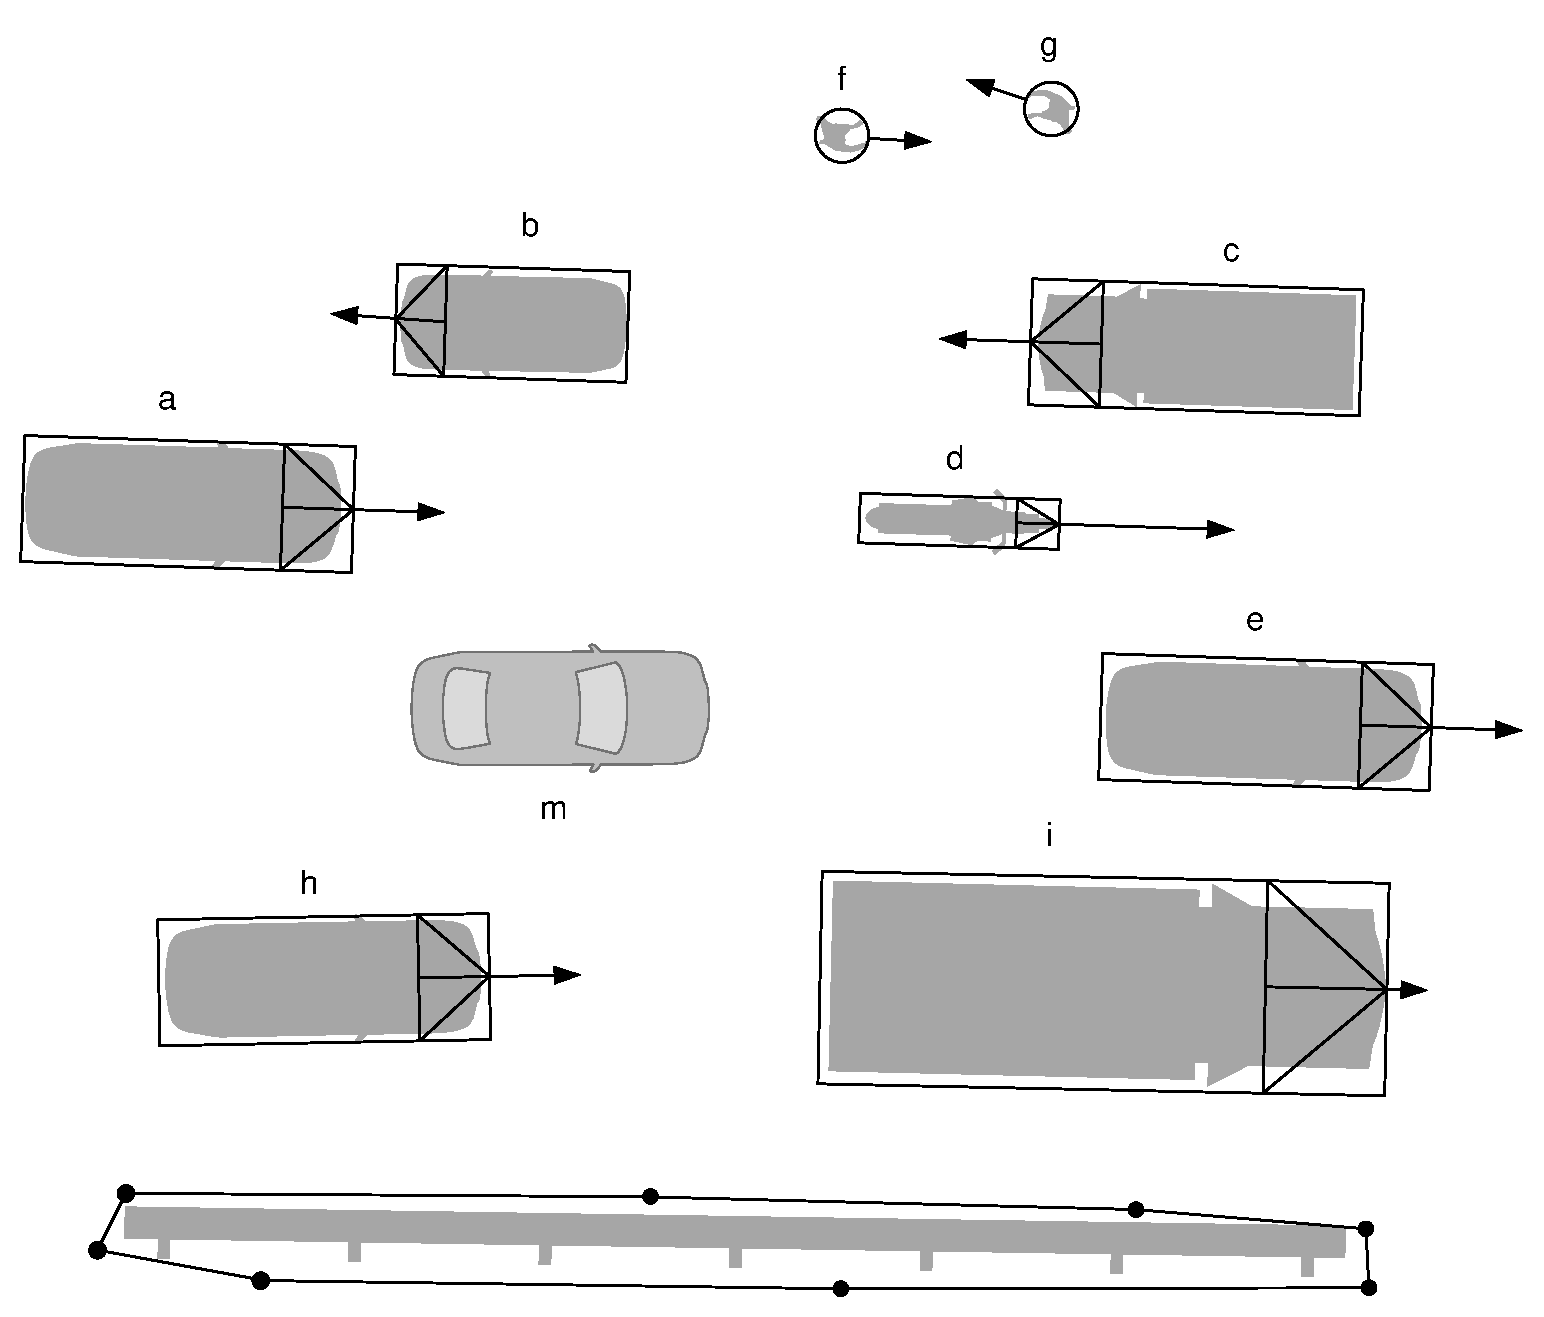
\includegraphics[width=.5\textwidth,clip, trim = 0cm 0cm 0cm 0cm]{2_Objektrepraesentation.eps}
	\hspace{.5cm}
	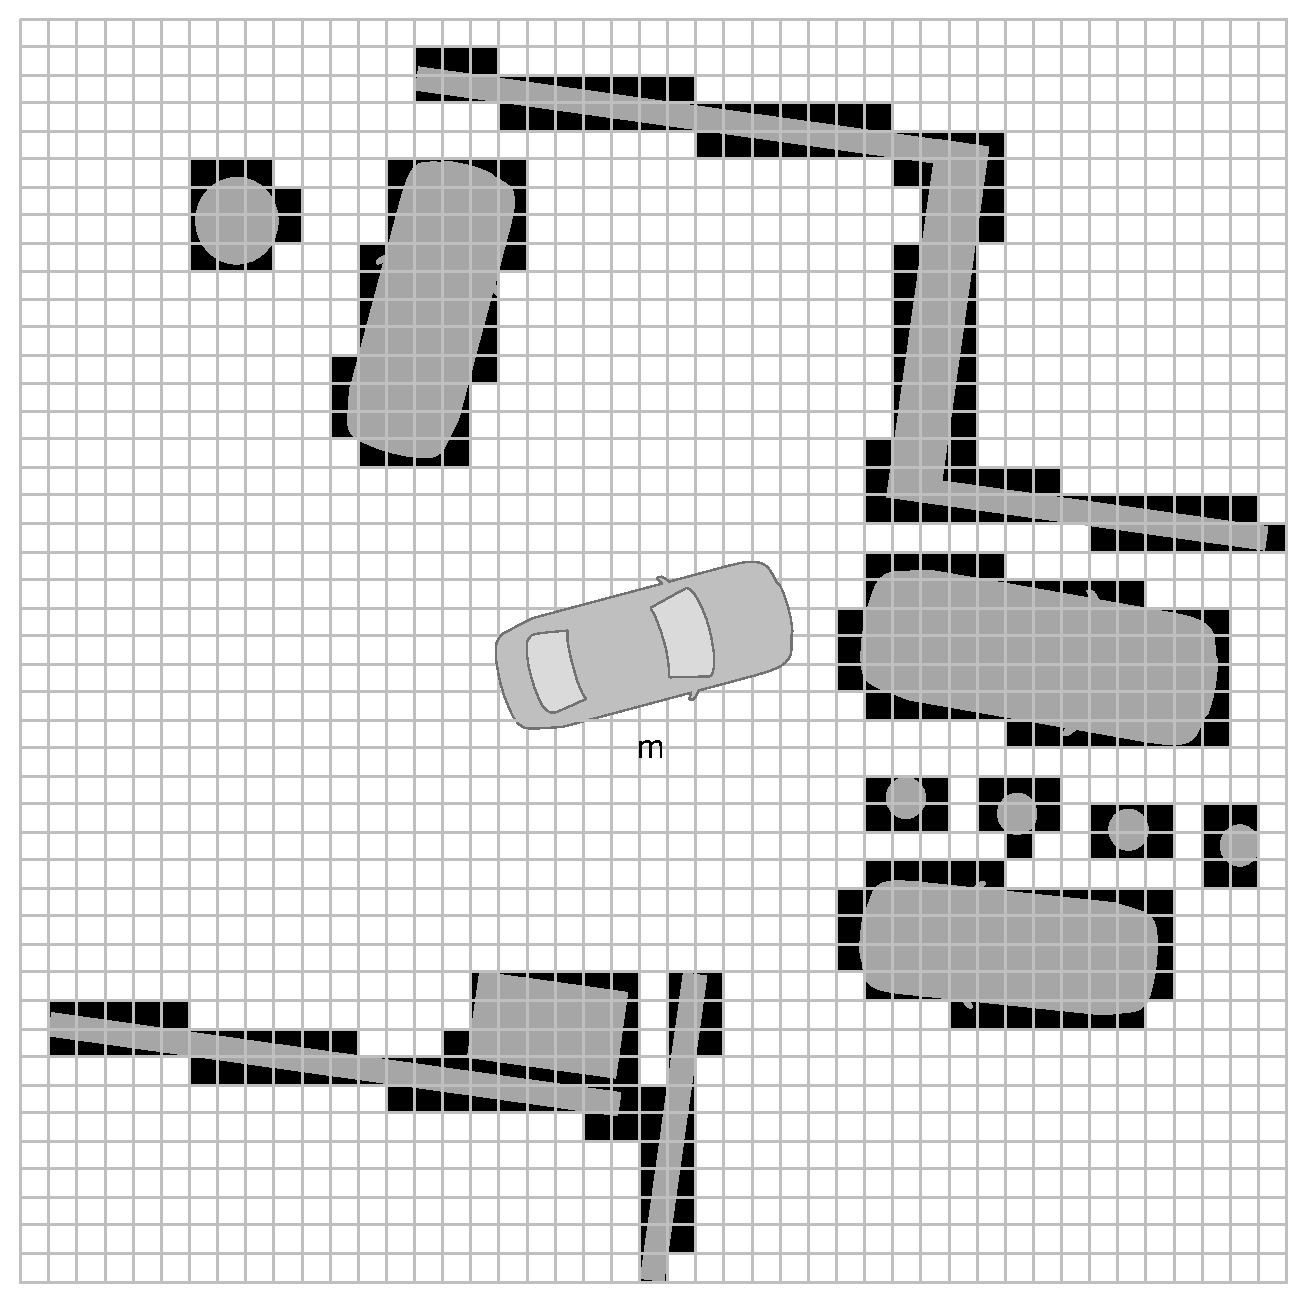
\includegraphics[width=.43\textwidth,clip, trim = 0cm 0cm 0cm 0cm]{2_Belegtheitskarte.eps}
 \caption[Repräsentationsformen des Fahrzeugumfelds]{Repräsentationsformen des dynamischen (links) und statischen (rechts) Fahrzeugumfelds mittels Objektlisten (links) und Belegungskarte (rechts), tatsächliche Objektabmaße in Grau}
 \label{fig:Objektrepraesentation}
\end{figure}

% Existenzwahrscheinlichkeit -> Konfidenzschwelle, Zustandunsicherheiten
% Situationsanalyse
% Fahrzeugumfelderfassung

\subsubsection{Umfeldprädiktion\index{Umfeldprädiktion}} \label{sec:praediction}
Aufgrund der immanenten Dynamik des Verkehrs erfordern aktive Fahreingriffe stets eine Situationsprädiktion. Begreiflicherweise reicht es nicht aus, erst während eines Aufpralls zu bremsen oder zu lenken. Im Vergleich zu den etablierten Methoden der Mehrobjektverfolgung steht jedoch die Entwicklung von Algorithmen zur Situationsprädiktion noch im Anfangsstadium. \\
Eine grobe Einteilung der bestehenden Prädiktionsalgorithmen kann über die Länge des Prädiktionshorizonts erfolgen. Handelt es sich um Prädiktionsverfahren innerhalb eines Sicherheitssystems, das erst kurz vor einer drohenden Kollision aktiv wird (s.\ \abschn{sec:systemactivation}), reicht es aus, die aktuelle Hindernisbewegung zu extrapolieren, z.B. unter der Annahme konstanter Längsbeschleunigungen und Fahrkrümmungen  \cite{Hillenbrand2006, Barth2008}. Soll der Prädiktionshorizont weiter erhöht werden, etwa für eine Assistenzfunktion im Stau, so ist es zielführend, den Verkehrsteilnehmern die Einhaltung der Straßenverkehrsordnung zu unterstellen. In \cite{ferguson2008detection, lawitzkyinteractive} und \citeltex{eichhorn2013Maneuverprediction} wird daher angenommen, dass sich Fahrzeuge langfristig entlang der Spur ausrichten und gleichzeitig so bremsen, dass Auffahrkollisionen vermieden werden. \\
Bei einem noch längeren Horizont (oder aber generell bei Fußgängern) wird häufig von \emph{Intentionserkennung} gesprochen und es überwiegt der stochastische Charakter des Prädiktionsproblems, sodass der zukünftige Aufenthaltsort der Verkehrsteilnehmer nur noch probabilistisch beschrieben werden kann, s.\ \zB \cite{borger2013fahrerintentionserkennung, rohrmuller2008probabilistic, lefevre2012risk, gindele2010probabilistic, althoff2009model, Althoff2010}.\\
Trotz des aktuellen Forschungscharakters ist langfristig, analog zum Umfeldmodell, mit einer zentralen Hindernisprädiktion innerhalb der Fahrzeugarchitektur zu rechnen, die die zukünftige Trajektorie eines jeden Umfeldobjekts permanent schätzt und den Assistenzfunktionen zur Verfügung stellt.



%Stichworte: 
% Umfeldmodell abstraktion: Typ, Abmaße, Position und Dynamikdaten
% Parameter und Zustandsschätzung
% Fehldetektionen und Falschdetektionen
% Bestrebung: Weg von Funktionsspezifischen Algorithmen hin zu einem Umfeldmodell, das bei unterschiedlichen Sensorkonfigurationen für verschiedene Funktionen hergenommen werden kann.
% Verkehrsszene
% Rendundanz bei Senrik bei HAF

 

% Der eigene Fahrzustand muss herangezogen werden um aufgrund der fahrezeugfesten Sensorik auf die Umwelt schließen zu können
\section{Systemaktivierung} \label{sec:systemactivation}
Da das Ein- und Ausschalten von Komfortfunktionen stets dem Fahrer überlassen ist, der abhängig von der Verkehrssituation entscheidet, wann ein System ihm assistieren soll, erfolgt das über eine sog.\ Benutzerschnittstelle \cite{lindberg2012entwicklung}, etwa über einen Knopf. Hierbei ist es dennoch wichtig, die Systemaktivierung und vor allem die -deaktivierung an zusätzliche Bedingungen zu knüpfen, die den technischen Grenzen des jeweiligen Systems Rechnung tragen und eine reibungslose Fahrerübernahme sicherstellen, s.\ \zB \cite{Schaller2008}. \\
Aktive Sicherheitssysteme stehen vor einer ganz anderen Herausforderung. Sie laufen permanent\footnote{Die meisten Sicherheitssysteme können dennoch vom Fahrer deaktiviert werden.} im Hintergrund, da sie ständig die Verkehrssituation  überwachen müssen, um bei gegebenem Anlass sofort mit aktorischen Interventionen zu reagieren. Beim Entwurf der Aktivierungsstrategie besteht nun die Schwierigkeit darin, den Eingriff auf der einen Seite so spät wie möglich vorzunehmen, um den Fahrer nicht ungerechtfertigter Weise zu bevormunden\footnote{Entsprechend der Wiener Straßenverkehrskonvention \cite{UnitedNations1993} gilt: "`\emph{Every driver shall at all times be able to control his vehicle or to guide his animals.}"'}, auf der anderen Seite so früh wie nötig einzuleiten, um eine Kollision zu verhindern. Stehen hierbei dem Assistenzsystem nicht dieselben Eingriffsmöglichkeiten (reduzierte Stellgliedanzahl, verminderter Dynamikumfang der Aktorik) wie dem Fahrer zur Verfügung, kann das in vielen Situationen nur kompromissbehaftet umgesetzt werden \cite{reinisch2012diss,dang2012steering}. Dieser Sachverhalt wird daher auch als sog.\ \emph{Eingriffsdilemma}\index{Eingriffsdilemma} bezeichnet.

Bevor ein kurzer Einblick in die algorithmische Herangehensweise der Aktivierung von Sicherheitssystemen gegeben wird, sei auf die Norm ISO 26262 \cite{ISO26262} hingewiesen, die allgemeine Entwicklungsmethoden der Funktionalen Sicherheit definiert  \cite{hillenbrand2011funktionale}. Sie stellt den Stand der Technik bei der Absicherung von sicherheitsrelevanten elektrischen/elektronischen Systemen in Kraftfahrzeugen dar und ist damit verbindlich vom Entwicklungsingenieur bei der Planung, Entwicklungsdurchführung und Validierung von Serienfahrerassistenzsystemen anzuwenden. Im Idealfall findet sie allerdings bereits im Forschungsstadium Berücksichtigung, da dann ein reibungsloser Ergebnistransfer in Richtung Serienentwicklung gewährleistet ist. \\
Zur Minimierung des verbleibenden Restrisikos (hier der aktivierten Assistenzfunktion) fordert die Norm unter anderem eine Sicherheitsintegrität des Systems, welche über sog.\ \emph{Automotive Safety Integrity Levels}\index{Automotive Safety Integrity Level} (ASIL) bewertet wird. Sie berechnen sich aus dem Schweregrad einer möglichen Verletzung, der Beherrschbarkeit der Fehlfunktion durch den Fahrer und der Häufigkeit der relevanten Fahrsituation. Je nach ASIL-Einstufung (A bis D) ergeben sich dann Konsequenzen für beispielsweise das Redundanzkonzept\index{Redundanz}, die formale Verifikation, die Selbstdiagnosefähigkeit, die Toleranzen oder die Komponententests des Assistenzsystems.

\subsection{Zustände einer unvermeidlichen Kollision} \label{sec:ics}
Die mobile Robotik beschäftigt sich seit jeher mit Algorithmen der Bewegungsplanung inmitten von Hindernissen, s.\ beispielsweise \cite{latombe1990robot, lavalle2006pa, fox1997dynamic, Fiorini1998}. Mit Hilfe sog.\ \emph{Konfigurationsraum}-Hindernisse\index{Konfigurationsraum} (kurz $\mathcal{C}$-Hindernisse) wird hierbei das Planungsproblem dahingehend vereinfacht, dass in den Hindernissen bereits die Abmaße des mobilen Roboters Berücksichtigung finden und der Roboter selbst auf einen Punkt reduziert werden kann. Für eine statische\footnote{Aufgrund der vereinfachten Repräsentation der beweglichen Hindernisse, etwa durch Rechtecke, ist es effizienter \cite{zieglerfastcollision2010, Lin1998}, die Kollisionsfreiheit einer konkreten Trajektorie innerhalb des Optimierungsalgorithmus hierarchisch abzuprüfen, anstelle die Konfigurationshindernisse für jeden Zeitschritt des Optimierungshorizonts komplett zu berechnen.} Umgebung erfolgt die Berechnung dieser $\mathcal{C}$-Hindernisse durch Einsatz von modernen Grafikkarten im Millisekundenbereich \cite{Tanzmeister2014ConfSpaceCosts}, wovon die in den Kap.\,\ref{chap:dynamische_Optimierung_dynamisch}, \ref{chap:dynamische_Optimierung_direkt} und \ref{chap:dynamische_Optimierung_indirekt} vorgestellten Algorithmen rechenzeittechnisch erheblich profitieren. \\
Die sog.\ Zustände einer unvermeidlichen Kollision \cite{fraichard2007short} (\emph{Inevitable Collision States}\index{Inevitable Collision States}, ICS), stellen gewissermaßen die Erweiterung der $\mathcal{C}$-Hindernisse dar. Sie beinhalten nämlich nicht nur die Geometrie des mobilen Roboters, sondern auch dessen \emph{zukünftige Modelldynamik}. Ein Robotik-System befindet sich nämlich genau dann in einem ICS, wenn, ganz gleich welche zukünftige Systemtrajektorie eingeschlagen wird, das System unweigerlich mit einem der Hindernisse kollidiert. \\
Für die Trajektorienplanung inmitten statischer und dynamischer Hindernisse bietet das ICS-Konzept einen ganz erheblichen Vorteil: Existiert eine effiziente ICS-Berechnung (ein sog.\ ICS-\emph{checker} \cite{martinez2009collision}), so reicht es für die Berechnung sicherer Trajektorien aus, vereinfacht gesprochen, die Überprüfung auf Kollisionen mit Hindernissen auf einem endlichen Horizont durchzuführen, wenn sichergestellt wird, dass der Trajektorien-Endpunkt nicht in einem ICS liegt \cite{fraichard2007short}, s.\ später Abschn.\,\ref{sec:stab_mpc}.
Aufgrund des erheblichen Rechenaufwands bei einer numerischen ICS-Berechnung, s.\ beispielsweise \cite{Lawitzky2014ICRA, falcone2011predictiveassessment, Karrenberg2008},  %aoude2010Threat, 
werden für die Fahrerassistenz stark vereinfachte Fahrzeugmodelle eingesetzt. So kann ein reines Bremsmanöver mittels Doppelintegrator mit beschränktem Eingang approximiert werden, wofür die 
ICS-Menge, wie in \abb{fig:ausweichen_vs_bremsen} dargestellt, analytisch berechnet werden kann. Soll zusätzlich die Querbewegung hinzugezogen werden, bietet sich die Approximation der Fahrzeugdynamik durch den sog.\ Kamm'schen Kreis\index{Kamm'scher Kreis} \cite{breuer20012bremsenhandbuch} an, s.\ \abb{fig:Beschleunigungskreise}.

%ICS kann herangezogen um Notbremsung auszulösen, und ausweichen zu planen (am Ende wieder in einem ICS) \cite{fraichard2007short}.
%	- Erweiterung des Dynamic Window Ansatzes
%	- ICS: Halber Tacho als Fußnote
%	ICS langfristig für HAF interessant: Erfassungshorizont endlich
	
%	- Berechnungsmethoden:
%	- Erreichbarkeitsmengen (mit Garantien)
%	- Monte-Carlo Simulationen
%	- Rückwärtsrechnen vom HIndernis
%	- Trajektorienplanung kann auch bei der Eingriffsstrategie helfen.
	
%	\cite{Althoff2010} % Diss

%\cite{falcone2011predictiveassessment} % Invarianten Mengen Volve invariant set theory von NMPC

%\cite{anderson2010optimal} % nmpc threat assesment


%\cite{Lawitzky2014ICRA}

%\cite{aoude2010Threat} % intersections Erreichbarkeitsmengen

%\cite{anderson2012constraint} % Hauptsächlich aktivierung mit minimalinvasiven manövern

\begin{figure}[h]
\centering
	\psfrag{I}[cc][cc]{ICS$_\text{Bremsen}$}
	\psfrag{J}[cc][cc]{ICS$_\text{Lenken}$}
	\psfrag{w}[tr][tr]{$\sqrt{-2 x a_\text{max}}$}
	\psfrag{u}[tr][tr]{$-x \sqrt{\frac{a_\text{max}}{2b}}$}
	\psfrag{h}[br][br]{Hindernis (0,0)}
	\psfrag{1}[cr][cr]{$v$}
	\psfrag{2}[tl][tl]{$x$}
	\psfrag{0}[cl][cl]{$v_c$}
\includegraphics[width=.9\textwidth,clip, trim = 0cm 0cm 0cm 0cm]{2_1d_ICS.eps}
\caption[Zustandsmenge einer unvermeidlichen Kollision durch Bremsen]{Zustandsmenge einer unvermeidlichen Kollision durch Bremsen (ICS$_\text{Bremsen}$, grau) des Systems $\dot x = v$; $\dot v = u \in [-a_\text{max}, a_\text{max}]$ zur Darstellung einer Auffahrsituation auf ein punktförmiges Hindernis im Ursprung; Im Vergleich dazu die (projizierte) Zustandsmenge einer unvermeidlichen Kollision durch konstante Querbeschleunigung (ICS$_\text{Lenken}$, schraffiert, Hindernisüberlappung $b$); Für Geschwindigkeiten unterhalb von $v_c$ kann bei Annäherung an das Hindernis zur Kollisionsvermeidung noch länger gebremst als ausgewichen werden, oberhalb von $v_c$ gerade umgekehrt, vgl.\ \cite{reinisch2012diss, schmidt2014fahrstrategien}.}
 \label{fig:ausweichen_vs_bremsen}
\end{figure}

		
		
\subsection{Subjektive Kritikalitätsbewertung\index{Kritikalitätsbewertung} des Fahrers} \label{sec:ttc} %empirisch
In den aktuellen Notbremsseriensystemen wird nicht erst dann gebremst, wenn eine Kollision unvermeidbar ist \cite{reinisch2012diss} und sich das Fahrzeug demnach in einem ICS befindet. Der Bestimmung des Eingriffszeitpunkts liegt nämlich eine andere, weniger konservative Überlegung zugrunde, die als Lösung eines Klassifikationsproblems angesehen werden kann. Aufgabe des Assistenzsystems ist demnach zu erkennen, ob der Fahrer überhaupt den potentiellen Kollisionspartner wahrgenommen hat oder nicht, und das möglichst früh. 
Da sich eine kamerabasierte Fahrerüberwachung bis dato nicht im Serieneinsatz befindet, % (s.\ auch \abschn{sec:grundlagen_bewertung}) 
müssen hierfür die Bremssysteme auf Basis der Relativbewegung zum Hindernis entscheiden, ob ein gewolltes Manöver oder ein Fahrfehler vorliegt. Als Bemessungsgrundlage (Klassifikationsmerkmal) hat sich vor allem die sog.\ \emph{time-to-collision}\index{time-to-collision}, kurz TTC, bewährt, welche die Zeit darstellt, die unter Beibehaltung der relativen Bewegungsdynamik zwischen den Kollisionspartnern bis zum Aufprall verbleibt. Sie repräsentiert nachweislich die vom Fahrer subjektiv wahrgenommene Kritikalität eines Auffahrmanövers. \\
Auch wenn die TTC ein breites Spektrum an Auffahrsituationen abdeckt, so berücksichtigt sie nicht die relative Position und Bewegung der Kollisionspartner quer zur Fahrtrichtung. So kann bei einer geringen Querüberlappung mit dem Hindernis der vermeintlichen Kollision durch eine minimale Lenkbewegung mühelos entgangen werden und das Manöver damit vom Fahrer gewollt sein. Um dies mit zu berücksichtigen, bietet sich als weiteres Kritikalitätsmaß die sog.\ \emph{time-to-steer}\index{time-to-steer} (TTS) an, also die Zeit, die verbleibt, bis der Fahrer durch Lenken spätmöglichst dem Unfall entgehen kann. Analog dazu definiert sich die \emph{time-to-brake}\index{time-to-brake} (TTB) oder kombiniert die \emph{time-to-react}\index{time-to-react} (TTR) \cite{Hillenbrand2006}. \\
In Bezug auf \abschn{sec:ics} stellt damit die TTC die zeitliche Distanz zu einem $\mathcal{C}$-Hindernis dar. Die TTR wiederum beschreibt nichts weiter als die verbleibende Zeit, bis sich das Fahrzeug in einem ICS befindet.



% - TTC: Warndilemma, da Reaktionszeit des Fahrers --> Aktive Eingriffe haben dieses Problem nicht. Ganz zu schweigen davon, dass der Fahrer die Warnung auch richtig interpretieren muss.

% Konfigurationsraum: berücksichtigt keine dynamik (alle Systemzustände) sondern nur position und Ausrichtung

% Ersatz für ICS: alle Zustände in denen ein Fahrer im Normalen fahrbetrieb sich nicht aufhält. KRitikalität

%Bremsen ist grndsätzlich sicherer als Ausweichen, weil Energie abgebaut wird.

%footnote: StvO ist so ausgelegt, dass immer einer vorfahrt hat und der andere gewähren muss: damit entsteht nich: Er denkt, dass ich denke, dass er denkt.
%Rückwirkungen des eigenen Fahrzeugs auf andere: Zumutbare verzögerungen in der Serie

%ICS liefern ein gutes Framework bestehende Assistenzsysteme und deren Auslösung zu interpretieren, neue Auslösekriterien zu erarbeiten und Trajektorienplanung für HAF sicherer zu gestalten.
		
	
		% Kreismethode
\begin{figure}[h]
	\psfrag{H}[cc][c][1.0]{Hindernis}
	\psfrag{a}[lb][lb][1.0]{$a_\text{max}t^2$}
	\psfrag{v}[tc][tc][1.0]{$v_0 \Delta t$}
\centering
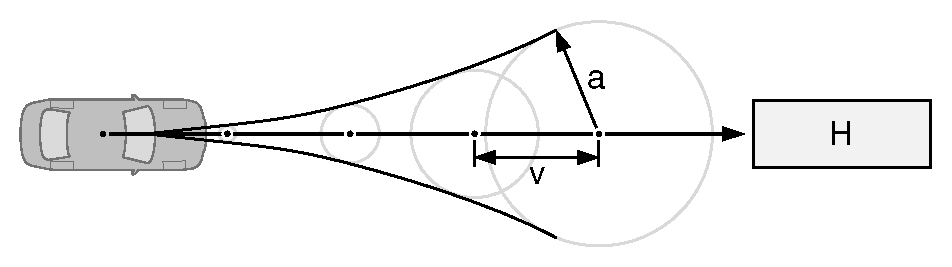
\includegraphics[width=1\textwidth,clip, trim = 0cm 0cm 0cm 0cm]{2_Beschleunigungskreise.eps}
 \caption[Erreichbare Schwerpunktpositionen]{Erreichbare Schwerpunktpositionen der durch maximale Beschleunigungen $a_\text{max}$ approximierten Fahrzeugdynamik \cite{schmidt2014fahrstrategien} (Kamm'scher Kreis \cite{breuer20012bremsenhandbuch}); Wie dem diagonalen Beschleunigungspfeil entnommen werden kann, beinhaltet die Erreichbarkeitsgrenze (schwarze Linie) beim Ausweichen immer auch eine Verzögerungskomponente, die jedoch in der Praxis häufig vernachlässigt wird.}
 \label{fig:Beschleunigungskreise}
\end{figure} 



% Abschätzungen über Physikalische Extrema: Kammscher Kreis

% Begriff: Deeskallationsmanöver


% Auslösung muss immer Wechselwirkungen berücksichtigen, wenn auch vereinfacht: Rückwärtiger Verkehr: zumutbare Verzögerung

% TTC kann auf als Merkmal für Lernende Verfahren sein.
% TTC verwendet Modell: z.B. konst. Geschwind., konst. Beschleun. etc.

% TTC: empirisch der Zusammenhang zur subjektiven Kritikalität

% Im Gegensatz dazu modelliert fTTR die physikalische Kritikalität; mit fTTR = 0 liegt z.B. der letztmögliche Zeitpunkt einer Deeskalation vor.

% neue algorithmen: Zeitliche Abfolge der Daten

% Althoff: Erreichbarkeitsanalyse


% Beispielbild: Berücksichtigung des Fahrbahnverlauf vs. geradeausfahren


% Fahrerinitiierte Systeme: Bremsassistent oder Ausweichassistent
% Automatisierte Eingriffe: Hohes Risiko

% TTC, TTR, TTB, TTS

% Physikalische Extrapolation (keine Prädiktion)

% rudimentär Prädiktion

% Fahrerüberwachung

% Unberechtigte Eingriffe, sog. Falschauslösungen (sportliche Fahrweise, Akzeptanz) müssen ebenso wie Fehlauslösungen vermieden werden.

% Fahrerreaktion muss berücksichtig werden -> Diss Reinisch

% Prädiktion anhand vorheriger Beobachtungen zu schätzen + Karte

% Unterscheidung: auf Manöverebene: Einscherer oder nicht, Abbieger etc.
% oder auf Trajektorienebene

% Einfachster Fall: TTC + Überlappung

% Algorithmik: Klassifikationsproblem

% Ausweichen vs. Bremsen: Eingriffsdillemma
% Falls auch autom. ausgewichen werden soll: Hindernis in der Fahrzeugmitte: Welche Richtung?
% Zusätzliche Probleme beim Ausweichen: Es muss auch wirklich frei sein. Bremsen macht immer das Richtige
% Kurzfristige Prädiktion: Es reicht sich auf die Physik zu verlassen: Es kann ja auch ein Fehler eines anderen Verkehrsteilnehmer vorliegen, sodass dieser selbst ein ander Fahrzeug rammt.
% Langfristige Situationsprädiktion muss wechselwirkungen zwischen den Verkehrsteilnehmern berücksichtigen

% Volvopaper: Welche Möglichkeiten hat der Fahrer?
% Inevitable Collision states

% Agentenbasierte Systeme?

% Methode sollte so schnell sein, dass sie auch zur Trajektorienplanung eingesetzt wird --> konstruktiv

% Monte Carolo simulationen

% Einhüllende

% Diskrete stochastische Systeme: Modellierung mittels Markov-Ketten

% Fahrer: hybrides system: Zustansübergänge mit kontinuierlichem Dynamik

% Stochastische Verifikationsmethoden

% Deterministishe Verifikation

% Kooperatives Umfeld (wird unterstellt), Verkehrsregeln geben die Abhängigkeit der reaktion zwischen den Hindernissen vor: Schwierigkeit: wie werden fehler erkannt?

% Modellierung: Gesamtverkehr stellt Systemzustand dar, der durch die Stellgrößen beeinflusst werden kann. Falls andere Fahrzeuge auf uns reagieren, dann sind auch ihr Trajektorien beeinflussbar. In manchen Situationen muss dies vorausgesetzt werden, da sonst eine Bremsung auf den vordermann eine kollision mit dem HIntermann zur folge hätte.

%\section{Optimierungskriterien und Koordinatenwahl}
%\subsection{Kartesische Koordinaten}
%\subsection{Frenet-Koordinaten}
%% Pfad vs. Trajektorie
%% Koordinatenwahl [XY, Frenet (Linearisierung um Traj.)]

\section{Bewertung} \label{sec:grundlagen_bewertung}
Die Beschreibung der Problemstellung aktiver Fahreingriffe des vorliegenden Kapitels erfolgt in zwei Teilen.
Der erste Teil leitet die interne Struktur eines Fahrerassistenzsystems her. Motiviert durch die beobachtbare Fahrweise routinierter Fahrzeugführer während hochdynamischer Manöver wird das klassische Drei-Ebenen-Modell derart modifiziert, dass es mit gesteigerter Fahrzeugbeherrschung einen immer größeren Teil des Fahrzustands auf der Führungsebene berücksichtigt. Die dort permanent zu lösende Aufgabe wird regelungstechnisch als Optimalsteuerungsproblem interpretiert, wodurch ein modellprädiktiver Regelkreis entsteht, der für die Stabilisierung des rückgeführten Teilfahrzustands zuständig ist. Die den Optimalsteuerungsproblemen zugrunde gelegten Optimierungskriterien berücksichtigen hierbei den Komfort, die Sicherheit und die Effizienz mit von Fahrer zu Fahrer unterschiedlichen Wichtungsfaktoren. \\
Die anschließende sog.\ Stabilisierungsebene wiederum wird als unterlagerter Regler betrachtet, wodurch im Zusammenspiel mit der modellprädiktiven Regelung ein kaskadierter Regelkreis entsteht, der auf der überlagerten Ebene den Optimierungskriterien des Manövers Rechnung trägt und auf der unterlagerten Ebene die spezifischen Eigenschaften des Fahrzeugs berücksichtigt.
%Neben den Standardsituationen wie Spur- und Abstandhalten erklärt der gegenüber dem Standardmodell modifizierten Systemaufbau auch die Unterstützung des Fahrers in Notfallsituationen ermöglicht, für welche eine permanente Optimierung des Fahreingriffs entsprechend der verfügbaren Fahrzeugdynamik und Umfeldinformation unabdingbar ist.

Zur Erleichterung der Übertragung des neuen Fahrermodells auf Fahrerassistenzsysteme und zur einheitlichen Betrachtung bestehender Algorithmen werden anschließend aus regelungstechnischer und robotischer Sicht die Begriffe \emph{Trajektorien-} und \emph{Bahnplanung}, \emph{Optimalsteuerung} sowie \emph{Optimale} und \emph{Modellprädiktive Regelung} erklärt und verglichen. 

Nach Darlegung der internen Grundstruktur einer Fahrerassistenz der Führungsebene, fokussiert der zweite Teil auf die dem System zur Verfügung stehenden Ein- und Ausgangsgrößen. Hierbei wird erkennbar, dass aus Entwicklersicht moderne Fahrzeuge im Hinblick auf die Möglichkeiten, die Fahrdynamik aktiv zu beeinflussen, kaum noch Wünsche offen lassen. Während zur Erprobung hochautomatisierten Fahrens noch vor einigen Jahren aufwändig Zusatzaktorik in die Versuchsträger eingebaut werden musste \cite{werivframe08, rauskolb2008caroline}, so reicht heute die Manipulation der Software des zuständigen Seriensteuergeräts aus, damit Lenkung, Gas und Bremse von extern angesprochen werden können. Mehr noch: Aufgrund der durchdachten Fahrzeugarchitektur stehen die detaillierten %in \abschn{sec:aktuatorik} 
Aktorikschnittstellen, namentlich das Sollhandmoment oder der -lenkradwinkel sowie das Antriebs- oder Bremsmoment am Rad, transparent zur Verfügung. Damit können die Fahrerassistenzfunktionen weitgehend unabhängig von der technischen Umsetzung der Stelleingriffe im jeweiligen Fahrzeug entworfen und leichter koordiniert werden, was den Entwicklungsprozess enorm beschleunigt und die Entwicklungskosten reduziert. \\
Dasselbe gilt für die zentrale Auswertung und Bereitstellung der erfassten Sensorinformationen. Auch wenn in aktuellen Serienfahrzeugen bestimmte Messgrößen wie die Gierrate (unnötiger Weise aus technischer Sicht) an mehreren Stellen im Fahrzeug von verschiedenen Teilsystemen erfasst werden, so lassen moderne Forschungsfahrzeuge %\cite{BMW_Autobahn, Daimler} 
eine klare Tendenz zu einer zentralen Informationsverarbeitung erkennen. Als Beispiel profitieren von einer verbesserten Schwimmwinkelschätzung dann zukünftig nicht nur das Elektronische Stabilitätsprogramm, sondern auf einen Schlag auch die Eigenlokalisierung, die Trajektorienberechnung, die Fahrzeugquerführung, die Mehrobjektverfolgung und die Situationsprädiktion. \\

Rückblickend auf den Wettkampf DARPA Urban Challenge 2007 kann aus heutiger Sicht festgehalten werden, dass ein Großteil der Kritik an den damaligen Ansätzen, s.\ \zB \cite{urmson2008adu, montemerlo2008junior, bacha2008odin, jfr2008}, ungerechtfertigt war. Hierzu zählt die Verwendung von Karteninformation, was unmittelbar mit der Abhängigkeit des Systems von einer entsprechend genauen Eigenlokalisierung verbunden ist (s.\ \abschn{sec:globalelok}). Nach heutigem Kenntnisstand ist nämlich eine Karte auf absehbare Zeit unverzichtbar, wenn es um die Realisierung einer Großzahl neuer Sicherheits- und Komfortfunktionen geht, sodass eisern an einer serientauglichen Eigenlokalisierung gearbeitet wird (s.\ ebenfalls \abschn{sec:globalelok}). Ein weiterer Kritikpunkt stellte die teils über mehrere Ebenen auf dem Dach angeordnete Rundumsensorik dar, die im Hinblick sowohl auf die Kosten als auch auf die Fahrzeugoptik aus Kundensicht inakzeptabel ist. Im Vergleich dazu unterscheiden sich aufgrund der unauffälligen Integration der Sensorhardware die heutigen Forschungsfahrzeuge der Hersteller von außen kaum noch von Serienfahrzeugen, bei teils gesteigerter Informationsgenauigkeit. Der Kostenaspekt einer umfangreichen Rundumsensorik bleibt jedoch, wie so häufig in der wettbewerbsgeprägten Automobilbranche, nach wie vor ein heikles Thema. Letztendlich entscheidet er darüber, ob sich ein Assistenzsystem langfristig rechnet.



%Dennoch hilft ein Grundverständis für die Funktionsweise der Einzelkomponenten, der Überlagerung mit dem Fahrer sowie deren Regelung bei der Modellierung und dem modellbasierten Reglerentwurf im Fahrerassistenzsystem, s.\ Kap.\,\ref{chap:stabilisierung}. 
% Fahrerüberwachung ganz wichtig für Vision zero
% c2x
% Rundumsensorik top
% Komfortfunktionen und Sicherheitsfunktionen nutzen dieselbe Sensorik
% Nachfolgende Kapitel: Gibt dem Entwickler für diese Aufgabe einen systematisierten Überblick über Methoden der Fahrzeugstabilisierung und Trajektorienoptimierung. Vorteilhafte Aufteilung in Regelung und Planung, Formulierung des Optimierungsproblems, Lösungsmethoden

%Aufteilung in bestehende/bewährte Stabilisierungsmethoden (ABS, DSC)

Zusammenfassend stehen damit aus Sicht der aktuellen Fahrerassistenzentwicklung von aktiven Fahreingriffen folgende drei Fragenstellungen im Mittelpunkt: 
\begin{itemize}
\item Welche nutzbringenden Sicherheits- oder Komfortfunktionen lassen sich auf Basis der bestehenden Aktorikschnittstellen mit der verfügbaren Sensorinformation umsetzen?
\item Welche Minimalanforderungen ergeben sich hierbei aus der anvisierten Fahrerassistenzfunktion an das Sensoriksetup?
\item In welche Richtung müssen Aktorik und Sensorik weiterentwickelt werden, um die angestrebte Funktionsqualität und -zuverlässigkeit zu realisieren?
\end{itemize}
An dieser Stelle sei an den kreativen Ingenieur und seine Arbeitsgruppe appelliert, neue Fahrerassistenzfunktionen nicht im Labor zu entwickeln. Vielmehr ist es zielführend, wenn der Forscher und Entwickler täglich mit offenen Augen in sein Fahrzeug steigt und sich dabei in die Lage unterschiedlicher Kunden versetzt. So kann aus einer erlebten Fahrsituation eine erste Funktionsidee entstehen, die in mehreren algorithmischen Iterationszyklen und Prototypen zu einer wertigen Assistenzfunktion heranreift. \\
Kreativität beruht jedoch zu großen Teilen auf Können. Auf es zielen die nachfolgenden Kapitel ab, indem methodisches Wissen in systematisierter Form vermittelt wird, welches sich, belegt anhand zahlreicher Literatur, in der Entwicklungspraxis aktiver Fahreingriffe als unverzichtbar herausgestellt hat. Die Kapitelinhalte beschränken sich insbesondere nicht auf die Darlegung der bloßen Theorie, sondern legen besonderen Wert auf die beispielhafte Beschreibung praktischer Umsetzungen. Somit wird der Leser befähigt, Parallelen zu neuen Fahrerassistenzfunktionen zu ziehen, damit er sie in vorteilhafter Weise mathematisch formulieren kann, um sie anschließend algorithmisch zu lösen und schließlich praktisch umzusetzen und zu erproben.

\cleardoublepage


% Zusammenfassung und Ausblick auf weiter Kapitel, s. z.B. Mikut Seite 237

%\begin{figure}[H]
	%\psfrag{0}[c][c][1.0]{$t_0$}
	%\psfrag{1}[c][c][1.0]{$t_1=t_0+\delta$}
	%\psfrag{2}[c][c][1.0]{$t_c=t_0+T_c$}
	%\psfrag{3}[c][c][1.0]{$t_p=t_0+T_p$}
	%\psfrag{4}[c][c][1.0]{Kontrollhorizont $T_c$}
	%\psfrag{5}[c][c][1.0]{Prädiktionshorizont $T_p$}
	%\psfrag{6}[c][c][1.0]{Vergangenheit}
	%\psfrag{7}[c][c][1.0]{\textbf{Prädiktion}}
  %\psfrag{a}[c][b][1.0]{Systemzustand x}
	%\psfrag{b}[c][c][1.0]{prädizierter Systemzustand $\bar{x}$}
	%\psfrag{c}[c][b][1.0]{Stellgröße u}
	%\psfrag{d}[c][b][1.0]{zu optimierende Stellgröße $\bar{u}$}
	%\centering
  	%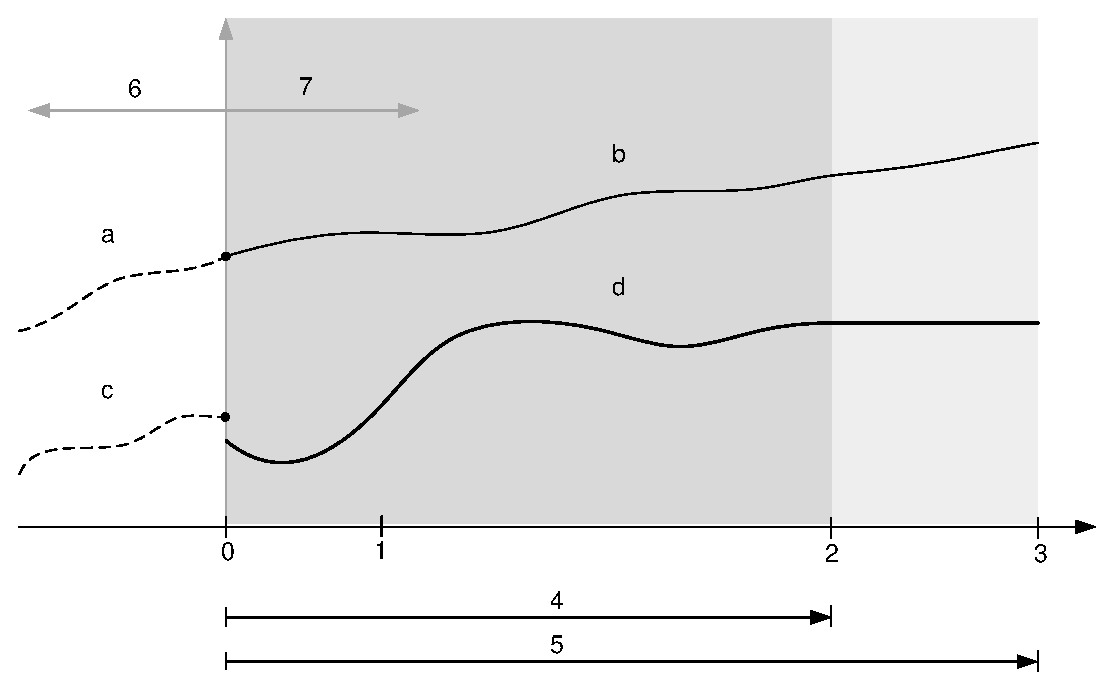
\includegraphics[width=1\textwidth,clip, trim = 0cm 0cm 0cm 0cm]{2_mpc_grundidee.eps}
		%\vspace{-0.1cm}
  	%\caption[Grundidee der modellprädiktiven Regelung]{Grundidee der modellprädiktiven Regelung, abgewandelte Darstellung nach \cite{Findeisen2002}}
    %\label{fig:grundidee_nmpc}
		%\vspace{-0.2cm}
%\end{figure} 

%\begin{figure}[H]
%\hspace{-0.9cm}
%\vspace{0.1cm}
	%\psfrag{1}[c][c][0.97]{\parbox[c]{7cm}{\begin{center}Lösungverfahren für die MPC\vspace{-0.08cm}\\ in der Optimalsteuerungsformulierung\end{center}}}
	%\psfrag{2}[c][c][0.97]{\parbox[c]{7cm}{\begin{center}Dynamische\vspace{-0.08cm}\\ Programmierung:\\\textit{\footnotesize Hamilton-Jacobi-Bellman-Gl.}\end{center}}}
	%%\psfrag{2}[c][c][0.97]{\parbox[c]{7cm}{\begin{center}Dynamische\vspace{-0.08cm}\\ Programmierung:\vspace{0.15cm}\\\textit{\footnotesize Hamilton-Jacobi-Bellman-Gl.\vspace{-0.15cm}\\ (Lockup-Table für Zustandsraum)}\end{center}}}
	%\psfrag{3}[c][c][0.97]{\parbox[c]{7cm}{\begin{center}Indirekte Methoden:\vspace{-0.08cm}\\ Minimumsprinzip von Pontryagin\\ \textit{\footnotesize Lösung mittels Variationsrechnung}\end{center}}}
	%\psfrag{4}[c][c][0.97]{\parbox[c]{7cm}{\begin{center}Direkte Methode:\vspace{-0.08cm}\\ Parametrisierung des Lösungsraums\vspace{0.15cm}\\ \textit{\normalsize\footnotesize Transformation in endlichdimensionales\vspace{-0.15cm} \\nichtlineares Optimierungsproblem}\end{center}}}
 %\psfrag{5}[c][c][0.97]{\parbox[c]{7cm}{\begin{center}Single Shooting\vspace{0.05cm}\\ \textit{\footnotesize Diskretisiert Steuervariablen\vspace{-0.15cm} \\(sequentiell)}\end{center}}}
 %\psfrag{6}[c][c][0.97]{\parbox[c]{7cm}{\begin{center}Kollokation\vspace{0.05cm}\\ \textit{\footnotesize Diskretisiert Steuer-\vspace{-0.05cm}\\ und Zustandsvariablen\vspace{-0.15cm} \\(simultan)}\end{center}}} 
 %\psfrag{7}[c][c][0.97]{\parbox[c]{7cm}{\begin{center}\vspace{0.05cm}Multi Shooting\vspace{0.05cm} \\ \textit{\footnotesize Diskretisiert Steuervariablen\vspace{-0.05cm} \\ und führt künstliche\vspace{-0.05cm} \\Zustandsvariablen ein\vspace{-0.15cm}\\ (simultan)}\end{center}}}
	%%\centering
		%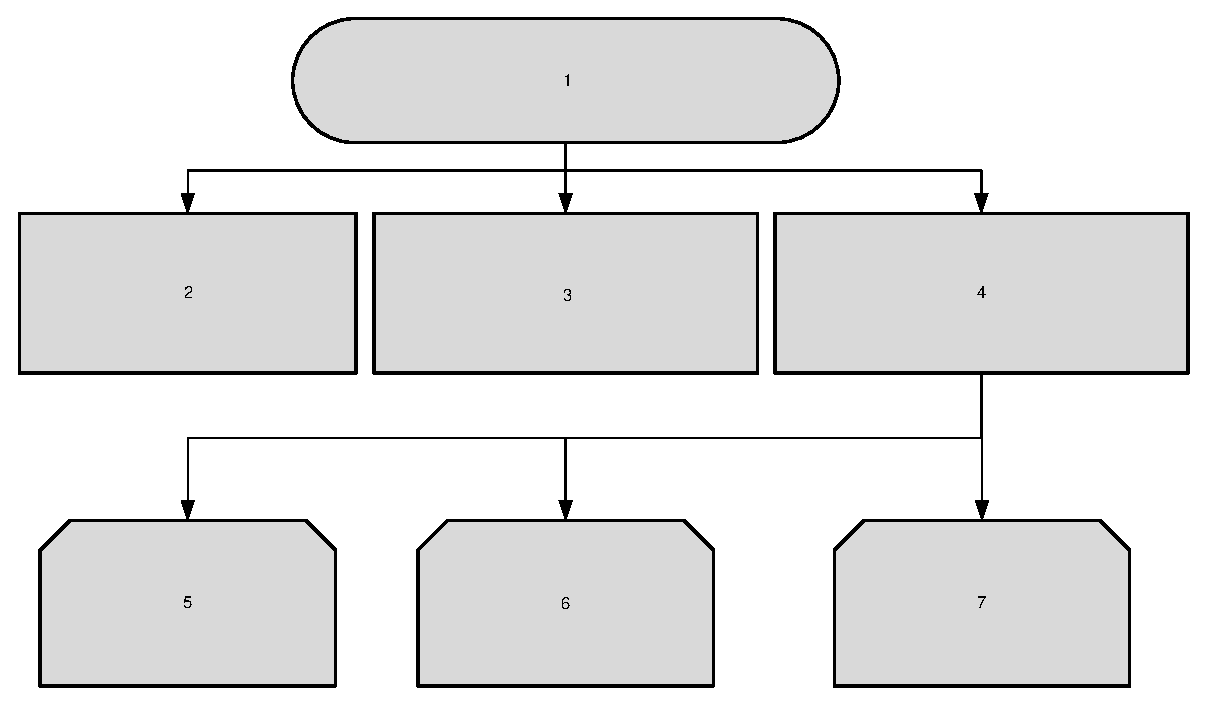
\includegraphics[width=1.11\textwidth,clip, trim = 0cm 0cm 0cm 0cm]{1_optimalsteuerung_uebersicht.eps}
	%\vspace{0.001cm}
	%\caption[Übersicht über die verschiedenen Zugänge zu Optimalsteuerungsproblemen]{Übersicht über die verschiedenen Zugänge zu Optimalsteuerungsproblemen,\\ abgewandelte Darstellung nach \cite{diehl_fast_multipleshooting}}
	%\label{fig:optimalsteuerung_uebersicht}
%\end{figure}



% Zustandsautomaten? Ist prinzipiell wichtig, da Teil eines jeden FAS
% Optimierung offline -> LUT
%	\section{Allgemeine Vorgehensweise}
% Best practice
% Iterativer prozess: modellierung evaluation, anpassung der modelle, nachhaltigkeit der entwicklung, viel simulation, modelle anwendung s abhängig, systemverständnis
% Binsenweisheiten, die nicht häufig genug wiederholt werden können, da sie immer noch falsch gemacht werden.
% Statischer, dynamischer Fahrsimulator
%	\subsection{Simulation}
%	\subsection{Fahrversuche}
	% 
%	\subsection{Absicherung}

% Hands-on-detection, Bewusst funktion schlechter machen um Missbrauch zu verhindern
% Probandenstudien, Expertentests

% Rausgeschmissen:
% % ISO 26262, Asil etc.
% Simulation, Fahrversuch, Prototypenbau, Probanden, Absicherung
% Aufbau eines Fahrerassistenzsystems

%	Entwicklungskriterien
% ZEISS-Punkte herein
% Statistische Auswertungen
% Nutzerakzeptanz
% Packaging (Angebotspakete)
% Cost Engeneering
% Diskretisierungsmethoden, Verweis auf folgende Kapitel
